%for a more compact document, add the option openany to avoid
%starting all chapters on odd numbered pages
\documentclass[12pt]{cmuthesis}

% This is a template for a CMU thesis.  It is 18 pages without any content :-)
% The source for this is pulled from a variety of sources and people.
% Here's a partial list of people who may or may have not contributed:
%
%        bnoble   = Brian Noble
%        caruana  = Rich Caruana
%        colohan  = Chris Colohan
%        comar    = Cyrus Omar
%        jab      = Justin Boyan
%        josullvn = Joseph O'Sullivan
%        jrs      = Jonathan Shewchuk
%        kosak    = Corey Kosak
%        mjz      = Matt Zekauskas (mattz@cs)
%        pdinda   = Peter Dinda
%        pfr      = Patrick Riley
%        dkoes = David Koes (me)

% My main contribution is putting everything into a single class files and small
% template since I prefer this to some complicated sprawling directory tree with
% makefiles.

% some useful packages
\usepackage{times}
\usepackage{fullpage}
\usepackage{graphicx}
\usepackage{amsmath}
\usepackage[numbers,sort]{natbib}
\usepackage[backref,pageanchor=true,plainpages=false, pdfpagelabels, bookmarks,bookmarksnumbered,
%pdfborder=0 0 0,  %removes outlines around hyper links in online display
]{hyperref}
\usepackage{subcaption}

\usepackage[capitalize,noabbrev,nameinlink]{cleveref}
\usepackage{float}
\usepackage[scaled]{inconsolata}

\captionsetup{labelfont=bf}
% \captionsetup{font=small}
\captionsetup{labelfont=bf}
\captionsetup{textfont={}}
%\captionsetup[subfloat]{font=small}
%\captionsetup[subfloat]{farskip=5pt}
%\captionsetup[subfloat]{captionskip=1pt}

\DeclareUnicodeCharacter{0097}{~}


% Approximately 1" margins, more space on binding side
%\usepackage[letterpaper,twoside,vscale=.8,hscale=.75,nomarginpar]{geometry}
%for general printing (not binding)
\usepackage[letterpaper,twoside,vscale=.8,hscale=.75,nomarginpar,hmarginratio=1:1]{geometry}

% Provides a draft mark at the top of the document. 
%\draftstamp{\today}{DRAFT}

\begin {document} 
\frontmatter

%initialize page style, so contents come out right (see bot) -mjz
\pagestyle{empty}

\title{ %% {\it \huge Thesis Proposal}\\
{\bf Filter Representation in Vectorized Query Execution}}
\author{Amadou Latyr Ngom}
\date{July}
\Year{2020}
\trnumber{}

\committee{
Andy Pavlo, Chair \\
Todd C. Mowry \\
}

\support{}
\disclaimer{}

% copyright notice generated automatically from Year and author.
% permission added if \permission{} given.

\keywords{Vectorization, Compilation, Filter, SIMD}

\maketitle

\begin{dedication}
\end{dedication}

\pagestyle{plain} % for toc, was empty

%% Obviously, it's probably a good idea to break the various sections of your thesis
%% into different files and input them into this file...

\begin{abstract}
Advances in memory capacity have allowed Database Management Systems (DBMSs) to store large amounts of data in memory, thereby shifting the performance bottleneck of query execution from disk accesses to CPU efficiency (i.e., instruction count and cycles per instruction). One technique used to achieve such efficiency in analytical applications is batch-oriented processing or \textit{vectorization}: it reduces interpretation overhead, improves cache locality, and allows for efficient loop optimizations (e.g., loop unrolling, SIMD vectorization). For each \textit{vector} (i.e., a batch of tuples), the DBMS needs to track the set of valid tuples after a predicate application. To that end, systems employ one of two data structures, or \textit{filter representations}: Selection Vectors (SelVecs) or Bitmaps. In this work, we analyze each approach's strengths and weaknesses to provide recommendations on how to implement vectorized operations. Through a wide range of micro-benchmarks, we determine that the optimal implementation strategy is a function of many factors: the cost of iterating through tuples, the cost of the operation itself, and how amenable it is to SIMD vectorization. Our analysis shows that Bitmaps perform better for operations that can be efficiently vectorized using SIMD instructions but that SelVecs perform better on all other operations due to a cheaper iteration logic.
\end{abstract}

\begin{acknowledgments}
I would like to thank my advisor Andy Pavlo for his guidance and help during my last two years at CMU. He has developed my interest in databases and computer science research in general and made my experience at CMU very educational and fun. I would also like to thank my amazing peers of the CMUDB group that helped me in this and other projects: Prashanth Menon, Matt Buttrovich, Wan Shen Lim, Lin Ma, Tanuj Nayak, Rohan Aggarwal, Gustavo Angulo, Tianyu Li, John Rollinson. Special shoutout to Prashanth Menon, whose help was invaluable in this project. Finally, I would like to thank my parents and siblings who guided and supported their son/little bro all throughout his life.
\end{acknowledgments}



\tableofcontents
\listoffigures
\listoftables

\mainmatter

%% Double space document for easy review:
%\renewcommand{\baselinestretch}{1.66}\normalsize

% The other requirements Catherine has:
%
%  - avoid large margins.  She wants the thesis to use fewer pages, 
%    especially if it requires colour printing.
%
%  - The thesis should be formatted for double-sided printing.  This
%    means that all chapters, acknowledgements, table of contents, etc.
%    should start on odd numbered (right facing) pages.
%
%  - You need to use the department standard tech report title page.  I
%    have tried to ensure that the title page here conforms to this
%    standard.
%
%  - Use a nice serif font, such as Times Roman.  Sans serif looks bad.
%
% Other than that, just make it look good...


\chapter{Introduction and Background}
\label{chapter1}
DBMSs typically handle two broad classes of applications: Online Transaction Processing (OLTP) and Online Analytical Processing (OLAP) applications. OLTP applications tend to be short-running, write-heavy queries that only touch a few entries in a database. OLAP applications are long-running, read-mostly queries that analyze large amounts of data. Due to the unique characteristics of each class, storage engines (i.e., the component of the DBMS stores the data), and query engines (i.e., the component that executes queries) must specialize storage formats and database algorithms to efficiently handle OLAP or OLTP applications \cite{one_size_fits_all}.  

OLTP applications aim for fast access and update on individual entries. Therefore, to improve cache performance, OLTP-specialized storage engines \cite{mysql,postgres,aurora,voltdb}, use a row-store (i.e., a storage format that stores all the attributes of an entry contiguously in memory and in cache). OLAP applications, on the other hand, optimize for fast reads and computing on attributes across multiple entries (e.g., to find the average value of an attribute across all tuples). OLAP-specialized storage engines \cite{redshift,vertica,saphana,duckdb}, thus, use a column-store (i.e., a storage format that stores similar attributes of different entries contiguously). Though most traditional DBMSs \cite{postgres,mysql} focused on OLTP applications and thus used row stores, column stores have resulted in significant performance gains for OLAP applications \cite{abadi_phd,one_size_fits_all}.

Besides the storage engine, disk-accesses were, historically,  the performance bottleneck of OLAP applications. For example, it takes around $1ns$ to perform random access in the  L1 cache, $100ns$ for DRAM, and $17000ns$ for SSDs \cite{numbersbyyear}. Disk accesses, thus, dominate the execution time of any query whose data is primarily disk-resident. Recent advances in DRAM manufacturing have exponentially decreased the price and increased the capacity of main-memory. The cost of DRAM per GB was around \$1000 in 2000, \$10 in 2010, and less than \$1 in 2020 \cite{dramprices}. This dramatic decrease in cost, and the corresponding increase in capacity, have both obeyed Moore's Law \cite{moorelaw}. It is now possible to store large databases entirely in DRAM. Rather than optimize for disk access, the query engines of in-memory DBMSs (i.e., DBMSs whose data fits in memory) must optimize for CPU efficiency by reducing instruction count and cycles per instruction when executing queries.

\begin{figure}[t!]
    \centering
    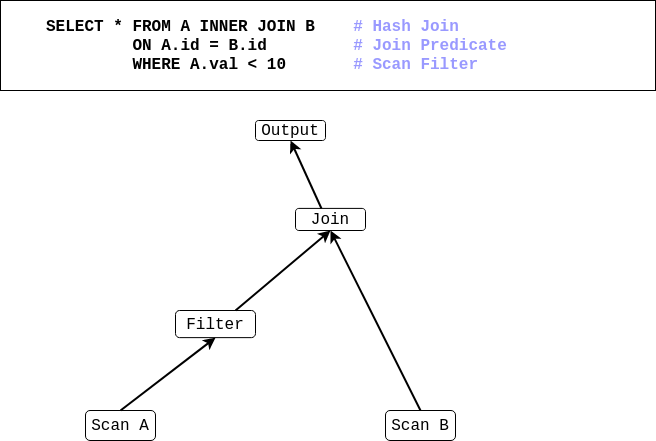
\includegraphics[scale=0.5]{images/SampleQuery.png}
    \caption{\textbf{Sample SQL Query and Plan.}}
    \label{fig:intro_query}
\end{figure}

\begin{figure}[t!]
    \centering
    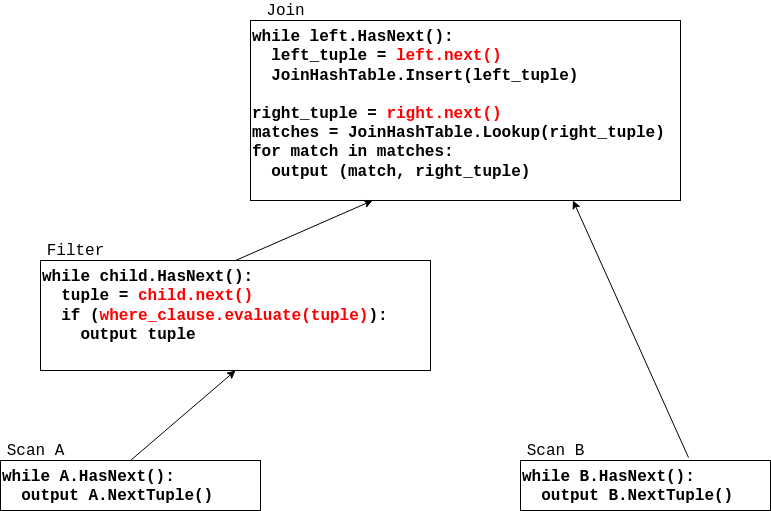
\includegraphics[scale=0.5]{images/Volcano.png}
    \caption{\textbf{The Iterator Model on the sample SQL query} -- The code in red indicates virtual function calls.}
    \label{fig:volcano_graph}
\end{figure}


The traditional query execution technique, the Iterator Model \cite{volcano}, is ill-suited for in-memory DBMSs due to CPU efficiency reasons. It executes a query by interpreting the query plan. In this model, each database operator implements a virtual \texttt{next()} function that returns the next tuple it can generate; each expression (i.e. addition, multiplication) also provides an virtual \texttt{evaluate()} function that takes in a tuple and returns a value. \cref{fig:volcano_graph} showcases the Iterator model with the sample query in \cref{fig:intro_query}. The operators \texttt{Scan A} and \texttt{Scan B} iterate through their respective tables and output the tuples to their parent operators. The filter only outputs tuples that satisfy the \texttt{WHERE} clause. The join first builds a hash table, then probes it to find matches. For every tuple -- of which there can be billions in an OLAP setting -- the virtual function calls (marked in red in the figure) constitute a significant overhead, which decreases CPU efficiency. Since the 2000s, there has been much work dedicated to optimizing the CPU efficiency of in-memory column stores for high-performance OLAP applications.

\citeauthor{monetdb2} proposed an alternative to the Iterator Model: the Materialization Model \cite{monetdb2}. In this model, rather than process and output one tuple at a time, each operator processes all its input tuples, then outputs all its results to the next operator. The authors also introduce specialized algorithms for each relational operator to exploit the columnar format of their system. Although the Materialization Model removes the Iterator Model's interpretation overhead, it can become memory-bound due to frequent materializations (e.g., copies) of large columns. To solve this issue, \citeauthor{boncz_vector} proposed a middle ground between the Materialization and Iterator Model: the Vectorization Model \cite{boncz_vector}. The thesis explores strategies for speeding up vectorized queries (i.e., queries executed using the Vectorization Model). As such, we will dedicate the rest of this chapter to an overview of the Vectorization Model. We discuss alternative query engine designs and optimizations for in-memory analytical DBMSs in \cref{chapter5}.

\section{The Vectorization Model}
\begin{figure}[t!]
    \centering
    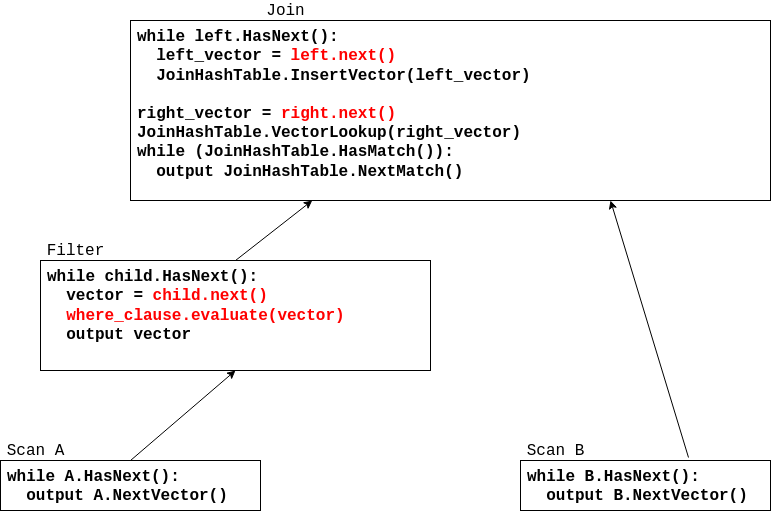
\includegraphics[scale=0.5]{images/Vectorization.png}
    \caption{\textbf{The Vectorization Model with the Sample Query} -- The code is nearly identical to that in \cref{fig:volcano_graph}, except that it processes vectors.}
    \label{fig:vectorization_graph}
\end{figure}

The Vectorization Model is almost identical to the Iterator model except that it operates on batches of $T$ tuples or \textit{vectors} (e.g., 2048 tuples at a time). The \texttt{next()} function returns vectors and the \texttt{evaluate()} function operates on vectors too. \cref{fig:vectorization_graph} showcases Vectorization Model on the sample query in \cref{fig:intro_query}; it is near identical to \cref{fig:volcano_graph}. The difference is that processing occurs one vector at at time rather than one tuple at a time.

\begin{figure}[t!]
\centering
\begin{subfigure}[t]{.5\textwidth}
 \centering
 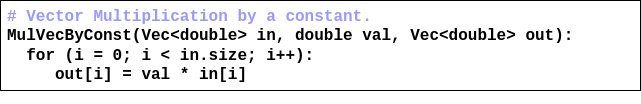
\includegraphics[width=0.9\textwidth]{images/MulByConstSISD.png}
 \caption{Unoptimized version.}
  \label{fig:vector_mul_sisd}
\end{subfigure}%
\begin{subfigure}[t]{.5\textwidth}
 \centering
 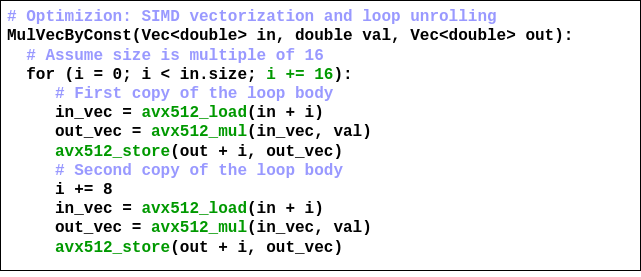
\includegraphics[width=0.9\textwidth]{images/MulByConstSIMD.png}
 \caption{Optimization version. There are two optimizations here: SIMD vectorization and loop unrolling with a factor of 2. The code in green indicates Intel's AVX512 instructions.}
  \label{fig:vector_mul_simd}
\end{subfigure}
\caption{\textbf{A Vectorized Multiplication Function} -- The programmer usually writes only the code on the left; the compiler can perform the optimizations on the right.}
\label{fig:vector_mul}
\end{figure}


This batch-oriented processing provides several benefits. First, virtual function calls occur for every $T$ tuples, which amortizes their overhead by a factor of $T$. Second, materializing $T$ tuples at a time instead of all tuples eliminates the memory pressure of the Materialization Model. Third, functions that operate on vectors, also known as \textit{vectorized primitives}, are usually amenable to loop optimizations (e.g., loop unrolling, SIMD vectorization) applied by either the compiler or the programmer. Consider, for a example, the primitive shown in \cref{fig:vector_mul_sisd}. It multiplies the elements in a vector by a constant number, and stores the result in a new vector. The loop of this primitive has independent iterations. Furthermore, the body of the loop only contains a load, a multiplication, and a store, which can all operate on SIMD vectors. As a result, the compiler or programmer can unroll and SIMD vectorize the loop. \cref{fig:vector_mul_simd} shows one way to optimize the loop. The body now contains AVX512 instructions \cite{intel2019} that perform that load, the multiplication, and the store, each operating on eight elements at a time. Besides, the loop unrolling (by a factor of two) optimization reduces the cost of loop maintenance.

Despite these benefits, the Vectorization Model introduces a new challenge. Individual tuples within a vector may be \textit{filtered out}, meaning that subsequent operators should not process them. For example, in \cref{fig:vectorization_graph}, the \texttt{Join} operator should not insert tuples that do no satisfy the \texttt{WHERE} clause in the \texttt{JoinHashTable}. It should only insert \textit{selected} tuples -- those not filtered out. Next, we discuss the methods used to identify selected tuples within a vector.

\section{Filter Representation}
\begin{figure}[t!]
    \centering
    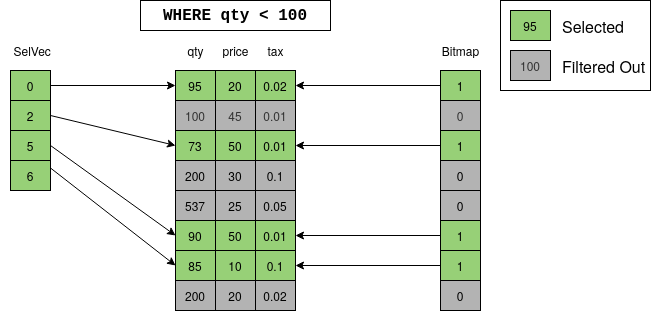
\includegraphics[scale=0.7]{images/FilterRepresentationIntro.png}
    \caption{\textbf{Filter Representation} -- Selection Vectors (left) index into selected tuples. Bitmaps (right) are only set on selected rows.}
    \label{fig:repr_intro}
\end{figure}

A \textit{filter representation} is the data structure used to identify selected tuples with a vector. \cref{fig:repr_intro} displays the two common representations: Selection Vectors (SelVecs) and Bitmaps. A SelVec stores a list of indices into the selected tuples. Tuples at an index stored within the SelVec are selected; tuples without an index are implicitly filtered out. A Bitmap, on the other hand, stores a list of bits. Its set bits indicate the selected tuples; its unset bits indicate filtered out ones. In the rest of this thesis, we will use the noun \textit{filter} to denote a particular instance of either data structure.


\subsection{Contribution}
Previous works on vectorized execution have chosen a filter representation strategy without providing an experimental comparison of the two approaches. Vectorwise \cite{vectorwise}, and works derived from it \cite{miro_adapt,everything_vectorized,sompolski_vec},  rely on SelVecs. IBM DB2's BLU \cite{ibm_blu} and the more recent VIP \cite{orestis_bitmap} rely on Bitmaps for the intermediary results of a table scan's \texttt{WHERE} clause filters, and SelVecs for other relational operators. Nonetheless, we find that supporting both representations, and dynamically choosing between them results in better performance than static implementations. Depending on the specific primitive and on the selectivity (i.e., the ratio of selected tuples) of its input vector, SelVecs can outperform Bitmaps and vice-versa. This work's main contribution is a methodology on how to optimize the performance of arbitrary vectorized primitives by taking into account filter representation, selectivity, and loop optimizations. We also provide recommendations for developers working on vectorized query engines on how to best implement primitives.

The remainder of this thesis is structured as follows. In \cref{chapter2}, we analyze the factors that influence the performance of vectorized primitive. We then derive insights for developers implementing vectorized query processing in \cref{chapter3}. Next, we use these insights on the OLAP queries of the TPCH \cite{tpch} benchmark and show the performance gains we obtain in \cref{chapter4}. Finally, we discuss related work in \cref{chapter5} and conclude in \cref{chapter6}.



\chapter{Computing on Filtered Vectors}
\label{chapter2}
The purpose of this chapter is to discuss the factors that influence the performance of vectorized primitives. We first categorize the kinds of operations that primitives perform and the possible ways to implement them. Afterward, we will present and explain the equation that quantifies the performance of each implementation. Finally, we raise the main questions whose answers, provided in \cref{chapter3}, will determine how to implement primitives optimally.

\section{Operations on Filtered Vectors}
\begin{figure}[t!]
\centering
\hspace*{\fill}%
\begin{subfigure}{.8\textwidth}
 \centering
 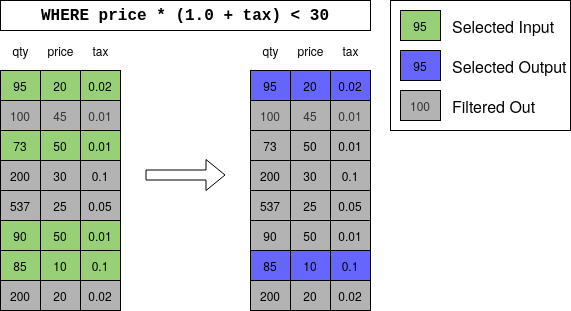
\includegraphics[width=0.9\textwidth]{images/UpdateIntro.png}
 \caption{Update operation.}
  \label{fig:update_intro}
\end{subfigure}%
\hspace*{\fill}%
\vspace*{8pt}%

\hspace*{\fill}% 

\begin{subfigure}{.8\textwidth}
 \centering
 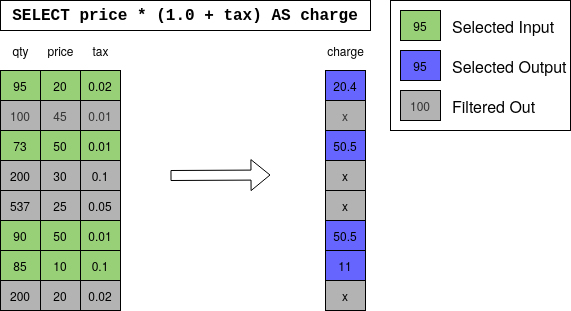
\includegraphics[width=0.9\textwidth]{images/MapIntro.png}
 \caption{Map operation.}
  \label{fig:map_intro}
\end{subfigure}
\caption{\textbf{Operations on Filtered Vectors} -- Updates change the set of selected tuple. Maps apply a function to the set of selected tuples without updating the set. Selected input tuples are in green. Selected output tuples are in blue.}
\label{fig:update_map_intro}
\end{figure}
\cref{fig:update_map_intro} shows the two kinds of primitives we seek to optimize: Updates and Maps. Updates apply a predicate function to the vector and modify the set of selected tuples accordingly. A scan filter (i.e., \texttt{WHERE} clause) is an example of an update operation. On the other hand, Maps keep the selected set but compute a new vector using a mapping function. A projection (i.e., \texttt{SELECT} clause) is an example of a map operation. There are other primitives, but these often have side-effects (e.g., insertion in a hash table for joins or an array for sorting) and are, therefore, not amenable to our optimizations for correctness reasons (e.g., Full Compute introduced in \cref{computestrategies}). As such, we focus on side-effect-free primitives.

\begin{figure}[t!]
    \centering
    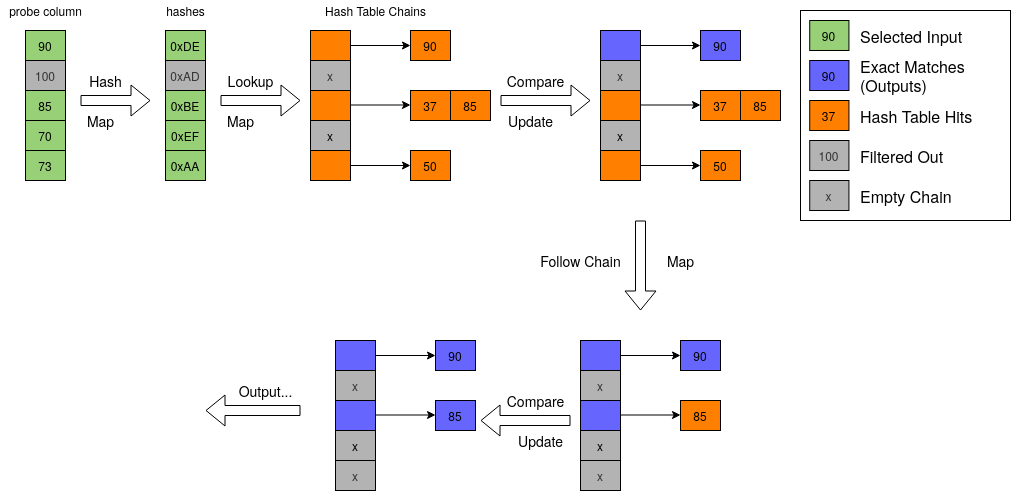
\includegraphics[scale=0.45]{images/NewJoinProbeExample.png}
    \caption{\textbf{Multi-Step Join Probe} -- The color green indicates selected items in the input vector. Orange indicates hash table lookup hits. Blue indicates exact matches after key comparison; these represent the output of the probe. Greyed out squares are filtered out tuples, or empty hash table chains.}
    \label{fig:probe_example}
\end{figure}
All relational operators are decomposable into a set of consecutive primitives. As mentioned above, simple relational operators like scan filters or projections consist of one individual primitive. Complex operators, like joins and aggregations, consist of multiple primitives. As a proof of concept, we showcase, in detail, the example of join probes in \cref{fig:probe_example}. The first primitive computes the hashes of the input tuples; the result is a vector of hash values. It is, therefore, a Map primitive. The second primitive performs a hash table lookup using the hashes to obtain a vector of hash table entries. It is also a Map primitive. Due to hashing collisions, the entries may not match the input, so the algorithm compares the join keys to filter out inexact matches. For example, key 90's hit in the hash table is an exact match, whereas key 73's is not. The third primitive performs this comparison; it is an Update primitive. The fourth primitive advances the hash table chains to obtain the next entries (e.g., 85 follows 37); it is a Map primitive. The probe then loops back to the comparison primitive to find exact matches (e.g., 85 now has an exact match). The set of exact matches constitutes the output of the join probe.

Other relational operators (e.g., aggregations) are similarly decomposable.

\section{Transitions}
\begin{figure}[t!]
    \centering
    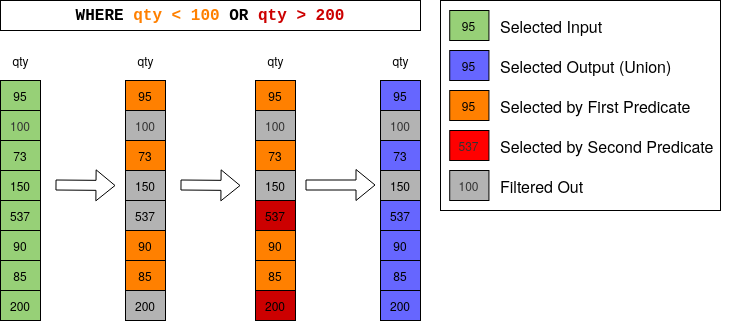
\includegraphics[scale=0.5]{images/DisjunctionHowto.png}
    \caption{\textbf{Decomposed Disjunctions} -- We apply the first clause (in orange) on all input tuples. In the second step, however, we only apply the second clause (in red) on those tuples that do not pass the first clause. In the third step, we take the union between the two outputs. The output tuples are in blue.}
    \label{fig:disjunctive_filter_howto}
\end{figure}

In between each primitive, operators may need to perform a \textit{transition} (i.e., modifications to the filter passed into the next primitive). We now discuss transitions and their associated cost. Most of the time, this cost is non-existent because the same filter is passed on to the next primitive: the transition is \textit{implicit}. For example, the hashing primitive and the lookup primitive in \cref{fig:probe_example} have the same filter; the transition performs no modifications. On the other hand, the Chain Following primitive operates on entries that do not satisfy the comparison: the transition involves a set difference. Set unions are another type of transition. Decomposed disjunctions \cite{pcq} (shown in \cref{fig:disjunctive_filter_howto}), for example, involve both set differences and unions. They decompose disjunctive \texttt{WHERE} clauses into a sequence of primitives -- one each for each conditional term. Each primitive operates on only tuples that have not satisfied the previous conditional terms, hence the set differences. The final filter consists of tuples that satisfy at least one primitive, hence the unions.

To the best of our knowledge, transitions are either implicit or take the form of set differences (for elements that do not pass the previous predicate) and unions (to obtain the final result). These operations are efficient to implement with Bitmaps by leveraging single-cycle bitwise AVX512 instructions \cite{intel2019} that operate on 512 bits at a time. Efficiently implementing set operations on SelVecs is more complicated.  Whenever necessary, Updates can write to one additional SelVec for tuples that do not pass the filter; this second SelVec implicitly corresponds to the result of a set difference. Note that it does not overlap with the first SelVec, so a union of any of their subsets is just an array append, a fast operation that can leverage SIMD instructions. 

To show that the overhead of these set operations is similar and negligible for both Bitmaps and SelVecs, we run an experiment that performs the decomposed disjunction shown in \cref{fig:disjunctive_filter_howto}. We synthetically generate the data so that each tuple has a $50\%$ chance of satisfying either conditional terms, the average case scenario. The data contains around $2000000$ tuples split into $1000$ vectors. The results are shown in \cref{fig:disjunctive_filter_perf}. The overheads are negligible; they are also nearly equal ($3.55\%$ and $4.06\%$ for Bitmaps and SelVecs, respectively). The representation, therefore, matters little when it comes to transitions. Given this, we will focus on optimizing primitives and will ignore transition costs.

\begin{figure}[t!]
    \centering
    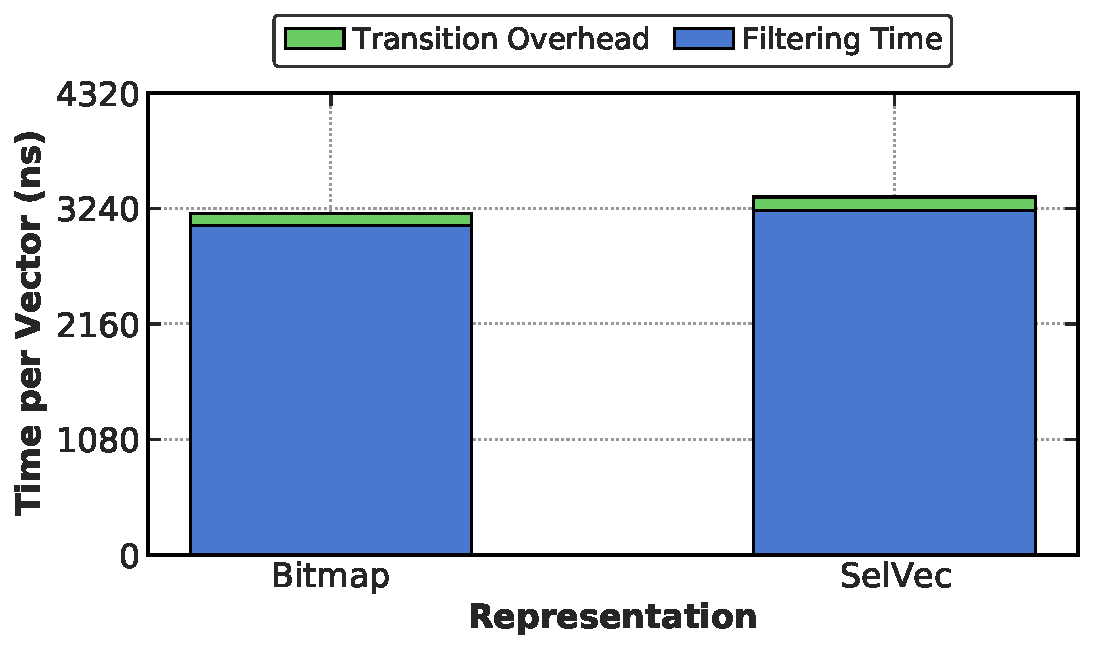
\includegraphics[scale=0.5]{eval/transition.pdf}
    \caption{\textbf{Transition Overheads} -- The overheads are $3.55\%$ and $4.06\%$ for Bitmaps and SelVecs respectively.}
    \label{fig:disjunctive_filter_perf}
\end{figure}


\section{Compute Strategies}
\label{computestrategies}
\begin{figure}[t!]
\centering
\hspace*{\fill}%
\begin{subfigure}{.8\textwidth}
 \centering
 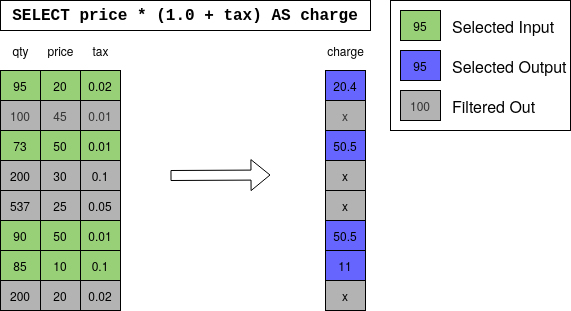
\includegraphics[width=0.9\textwidth]{images/SelectiveCompute.png}
 \caption{Selective Compute. An \texttt{x} indicates an uninitialized value.}
  \label{fig:compute_intro_selective}
\end{subfigure}%
\hspace*{\fill}%
\vspace*{8pt}%

\hspace*{\fill}% 

\begin{subfigure}{.8\textwidth}
 \centering
 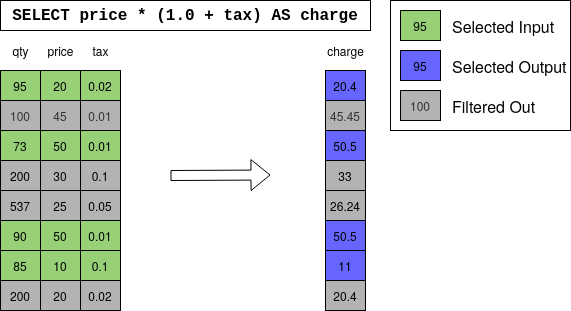
\includegraphics[width=0.9\textwidth]{images/FullComputeMap.png}
 \caption{Full Compute. There are no uninitialized values}
  \label{fig:compute_intro_full}
\end{subfigure}
\caption{\textbf{Compute Strategies}}
\label{fig:compute_intro}
\end{figure}


A compute strategy determines the implementation of Map and Update primitives. We consider three compute strategies: (1) Selective, (2) Full, and (3) Mixed Compute. Selective Compute only applies the given functions on selected tuples, whereas Full Compute applies them on all tuples. \cref{fig:compute_intro} shows each approach's effect. The Selective Compute strategy (\cref{fig:compute_intro_selective}) leaves undefined values because it does not operate on filtered out entries, whereas the Full Compute strategy (\cref{fig:compute_intro_full}) operates of every tuple and thus produces a result for each. As we show in \cref{chapter3}, although Full Compute usually performs more work, it benefits from SIMD vectorization, simple loop structure (for loop unrolling and interleaving), and easy branch prediction. To exploit this trade-off, the third strategy, Mixed Compute, switches from Full Compute to Selective Compute when the selectivity (i.e., the ratio of selected tuples) goes below a threshold. The next chapter will show how to derive this threshold experimentally.

\begin{figure}[t!]
    \centering
    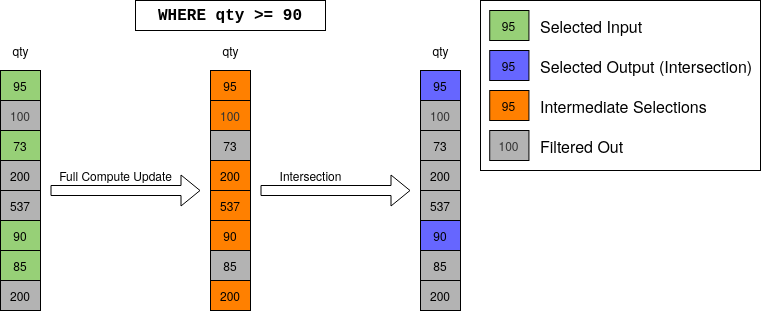
\includegraphics[scale=0.5]{images/FullComputeUpdate.png}
    \caption{\textbf{Update with Full Compute} -- The leftmost vector is the input vector; its selected elements are shown in green. The middle vector is the intermediary output of the full compute; its selected elements are shown in orange. The last vector has the intersection of the input filter and the intermediary filter; its selected elements are shown in blue.}
    \label{fig:full_compute_update}
\end{figure}


On Update primitives, Full Compute first finds the set of all tuples in the vector that pass the predicate, regardless of the input filter. The final filter is the intersection of this intermediary filter and the input filter. This process is shown in \cref{fig:full_compute_update}. Notice how the intermediary filter contains elements filtered out of the input vector (e.g., 100 and 200). The intersection is, thus, necessary to remove these elements from the final output. Bitmap intersection is efficient thanks to the AVX512 \texttt{and} instruction that intersects 512 bits in one cycle \cite{intel2019}, but SelVecs require a slow intersection of sorted sets \cite{sorted_set}. Thus, Full Compute is not efficiently compatible with SelVecs on Update primitives. This incompatibility will become important when choosing a strategy to implement.

\begin{figure}[t!]
\centering
\hspace*{\fill}%
\begin{subfigure}[t]{.8\linewidth}
 \centering
 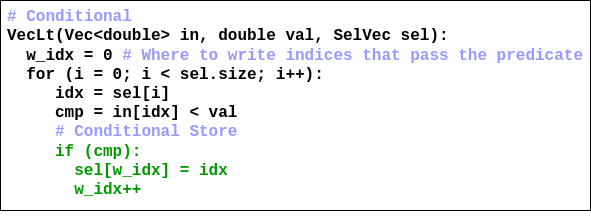
\includegraphics[width=0.9\linewidth]{images/ConditionalStoreConditional.png}
 \caption{Conditional Store. We only update the SelVec when the condition is satisfied (code in green).}
  \label{fig:conditional_store}
\end{subfigure}%
\hspace*{\fill}%
\vspace*{8pt}%

\hspace*{\fill}% 

\begin{subfigure}[t]{.8\linewidth}
 \centering
 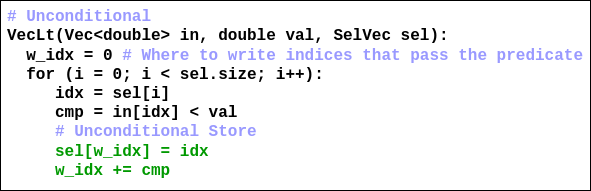
\includegraphics[width=0.9\linewidth]{images/ConditionalStoreUnconditional.png}
 \caption{Unconditional Store. We always update the SelVec regardless of the condition (code in green). The condition determines whether to increment the write index or not.}
  \label{fig:unconditional_store}
\end{subfigure}
\caption{\textbf{Conditional versus Unconditional Store} -- Both listings select the elements within the input vector (first parameter) that are less than the second parameter. Initially, the SelVec (third parameter) contains selected indices of the input vector. In the end, it only contains those that pass the predicate.}
\label{fig:conditional_selvec}
\end{figure}

Furthermore, for Updates with SelVecs, there is another implementation decision: Conditional versus Unconditional Store. \cref{fig:conditional_selvec} shows these options. Both primitives attempt to select the values less than a given input constant. They differ only in how they update the SelVec (code in green). The Conditional Store (\cref{fig:conditional_store}) updates the SelVec when the condition is true. The Unconditional Store (\cref{fig:unconditional_store}) always the updates the SelVecs, but only increments the write index when the condition is true. We do not focus on this decision, for it has been studied extensively before \cite{miro_adapt, sompolski_vec}. Previous work identified branch mispredictions costs as the main factor influencing this decision. The Conditional Store implementation is competitive when the same branch is taken around $90\%$ of the time or more, meaning that less than $10\%$, or more than $90\%$ of tuples satisfy the condition. All the experiments in this thesis use the optimal strategy on Update primitives that use SelVecs.

Given a compute strategy and a filter representation, the next section provides a framework for analyzing the performance of any vectorized primitive.

\section{Primitive Performance}
\label{prim_perf_section}

\begin{figure}[t!]
\centering
\hspace*{\fill}%
\begin{subfigure}{.8\textwidth}
 \centering
 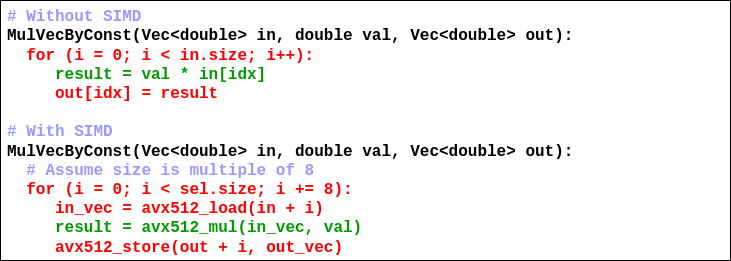
\includegraphics[width=0.9\textwidth]{images/RationaleMapFull.png}
 \caption{Full Compute. This function iterates through all elements, including filtered out ones.}
  \label{fig:rationale_full}
\end{subfigure}%
\hspace*{\fill}%
\vspace*{8pt}%

\hspace*{\fill}%  
\begin{subfigure}{.8\textwidth}
 \centering
 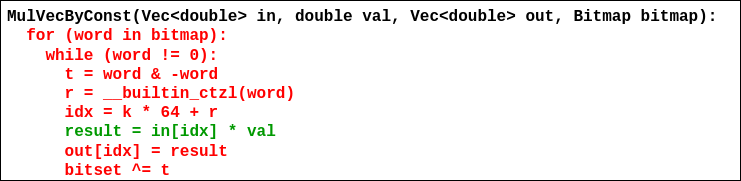
\includegraphics[width=0.9\textwidth]{images/RationaleMapBitmap.png}
 \caption{Selective Compute with a Bitmap. The iteration logic is adapted from \cite{bitmap_iteration}. The logic is not amenable to SIMD vectorization.}
  \label{fig:rationale_bitmap}
\end{subfigure}%
\hspace*{\fill}%
\vspace*{8pt}%

\hspace*{\fill}%  
\begin{subfigure}{.8\textwidth}
 \centering
 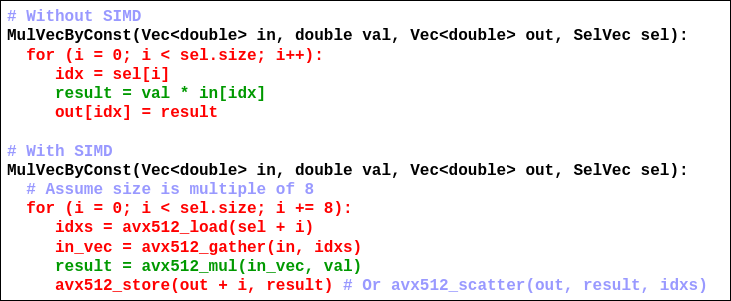
\includegraphics[width=0.9\textwidth]{images/RationaleMapSelVec.png}
 \caption{Selective Compute with a SelVec. Reading an element involves an indirection to first obtain its index. In the SIMD code, the \texttt{gather} instruction handles this indirection. The last \texttt{scatter} is only necessary to maintain consistent indices between the input and output vector during multi-step Map operations. It should otherwise be avoided due to its slowness.}
  \label{fig:rationale_selvec}
\end{subfigure}
\hspace*{\fill}%
\vspace*{8pt}%

\caption{\textbf{Implementing Vector Primitives} -- The code in green indicates the core operation (multiplication). The code in red indicates iteration logic.}
\label{fig:rationale_code}
\end{figure}

This section analyzes the performance of primitives according to their implementations. Our primitive implementations follow one of the patterns shown in \cref{fig:rationale_code}. This listing shows the strategies to multiply a vector by a constant (a Map primitive) along with their optimized versions using SIMD instructions: Full Compute (which does not depend on representation), Selective Compute with SelVecs, and Selective Compute with Bitmaps. In each instance, the code is a loop divided in two parts: the \textit{iteration logic} (code in red), and the \textit{core operation} (code in green). The core operation (e.g., multiplication by a constant) is independent of the strategy. On the other hand, the iteration logic is strategy dependent; it determines how to iterate through tuples -- whether selected ones in the case of Selective Compute or all tuples in the case of Full Compute -- to perform the core operation and store its result.

\begin{figure}[t!]
    \centering
    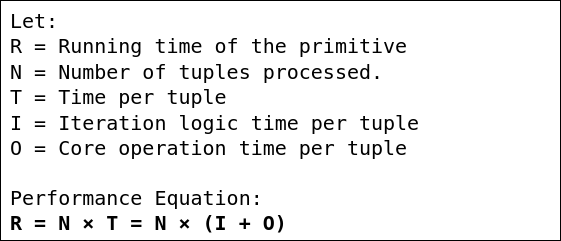
\includegraphics[scale=0.5]{images/PerfEq.png}
    \caption{\textbf{The Primitive Performance Equation}}
    \label{fig:perf_equation}
\end{figure}


The equation in \cref{fig:perf_equation} shows the formula to compute the running time of a primitive. The first equality indicates that the total running time is equal to the number of tuples processed multiplied by the time spent per tuple. The second equality splits the time spent per tuple in two: the time dedicated to the iteration logic, and the time dedicated to the core operation. This formula provides a framework to analyze any vectorized primitive. Let us consider how each of the three factors in the second equality relates to implementation strategies.

\textbf{Number of Tuples Processed}: Selective Compute processes only selected tuples; Full Compute processes every tuple. Thus, the lower the selectivity (i.e., the ratio of selected tuples), the more wasteful Full Compute is.

\textbf{Iteration Logic Time per Tuple}: Full Compute, while processing more tuples, has the simplest iteration logic because it does not aim to identify the selected ones. For Selective Compute, iterating over a Bitmap (e.g., \cref{fig:rationale_bitmap}) is more expansive than iterating over a SelVec (e.g., \cref{fig:rationale_selvec}) because of the bit operations required by Bitmaps. Optimizations like loop unrolling and SIMD vectorization can further decrease the iteration logic time per tuple, but they are only available for Full Compute and SelVecs. The Bitmap's selective iteration logic is too complex to perform such optimizations.


\begin{figure}[t!]
\centering
\hspace*{\fill}%
\begin{subfigure}[t]{.8\linewidth}
 \centering
 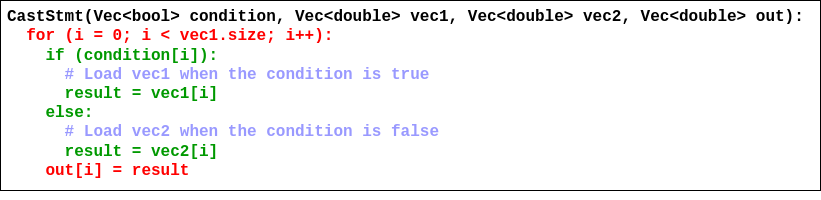
\includegraphics[width=0.9\linewidth]{images/BranchingCodeSISD.png}
 \caption{SISD code.}
  \label{fig:branching_sisd}
\end{subfigure}%
\hspace*{\fill}%
\vspace*{8pt}%

\hspace*{\fill}% 

\begin{subfigure}[t]{.8\linewidth}
 \centering
 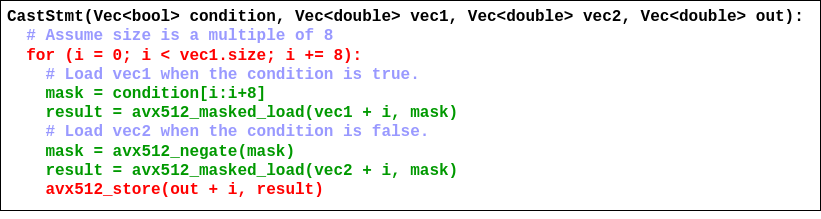
\includegraphics[width=0.9\linewidth]{images/BranchingCodeSIMD.png}
 \caption{SIMD code.}
  \label{fig:branching_simd}
\end{subfigure}
\caption{\textbf{SISD Branching Code versus SIMD} -- Both listings select elements from one of \texttt{vec1}, or \texttt{vec2} depending on the \texttt{condition}. In the SISD code, only one branch is executed every iteration. In the SIMD code, we rely on masking to select which vector to load from, but all instructions are executed at every iteration.}
\label{fig:branching_code}
\end{figure}


\textbf{Core Operation Time per Tuple}: The core operation is the same for all strategies. The only way to reduce its contribution to the running time is through data-parallel SIMD instructions, which are only available with Full Compute and Selective Compute with SelVecs. There are, however, situations where SIMD vectorization provides little gain or even hurts performance. Consider the example in \cref{fig:branching_code}. This function selects an element from one of two vectors depending on the value in a third boolean vector. It corresponds to a relational \texttt{CASE} statement. For each loop iteration, the SISD code (\cref{fig:branching_sisd}) only executes one branch. The SIMD code (\cref{fig:branching_simd}) executes all branches and relies on SIMD masking to set the correct vector lanes; it ends up executing more instructions that the SISD code, which reduces the benefits data-parallelism. In general, core operations benefit most from SIMD vectorization when they only contain straight-line (i.e., no branches), arithmetic, and bitwise instructions.

The explanation above raises three questions that can allow us to determine the optimal strategy for any primitive: What is the input vector's selectivity? Can we use data-parallelism to perform the core operations on multiple elements at a time? Does the core operation contain instructions that make data-parallelism inefficient (e.g., branching)? The next chapter experimentally derives the best strategies according to the answers to these questions.

\chapter{Optimal Strategies}
\label{chapter3}
In this chapter, we aim to derive the optimal execution strategy for any given primitive experimentally. In doing so, we will provide a decision tree that developers can use to guide the implementation of vectorized primitives.

\begin{table}[t!]
\centering
\begin{tabular}{|l|l|l|l|l|}
\hline
\textbf{Strategy Name} & \textbf{Representation} & \textbf{Compute} & \textbf{SIMD}      & \textbf{Compatibility} \\ \hline
SelVecPartial         & Selection Vectors       & Selective        & None               & Update and Map         \\ \hline
SelVecManual          & Selection Vectors       & Selective        & Manually Written   & Update and Map         \\ \hline
BitmapPartial         & Bitmaps                 & Selective        & None               & Update and Map         \\ \hline
BitmapFull            & Bitmaps                 & Full             & Auto Vectorization & Update and Map         \\ \hline
BitmapFullManual      & Bitmaps                 & Full             & Manually Written   & Update and Map         \\ \hline
Full                  & Either                  & Full             & Auto Vectorization & Map                    \\ \hline
FullManual            & Either                  & Full             & Manully Written    & Map                    \\ \hline
\end{tabular}
\caption{\textbf{Implemented Strategies} -- For the SIMD columns, `Auto Vectorization' indicates that we rely on compiler auto vectorization, whereas `Manually written' indicates that we write SIMD code ourselves using intrinsics. On the compatibility column, Update operations cannot use both Full Compute and Selection Vectors, which explains the last two entries.}
\label{tab:strategies}
\end{table}


The chapter is divided into a series of experiments based on the questions raised in \cref{prim_perf_section} to determine the optimal strategy for a given primitive. \cref{tab:strategies} summarizes all the strategies we implemented. As noted before, there is no Full Compute strategy for Updates that works with SelVecs. Update experiments will thus always use a Bitmap for Full Compute; For Map experiments, the representation is irrelevant because Full Compute neither reads nor updates the filter. In addition to relying on compiler auto-vectorization, we also experimented with manual vectorization (e.g., with SelVecManual) for straight-line arithmetic and bitwise operations (as in \cref{sldpsection}).

We run the experiments on an Intel Xeon Platinum 8124M CPU @ 3.00GHz with AVX512 support. We use the NoisePage DBMS \cite{noise_page}, with a read-only column store as its storage engine, compiled with clang version 9 \cite{clang}.

In each experiment, we synthetically generate the data and manually vary the selectivity of each primitive's input vector from $0.0$ to $1.0$ in increments of $0.05$ to show the impact selectivity has on what the optimal strategy is. For example, we set a random $25\%$ of bits in a Bitmap to obtain filter with a selectivity of $0.25$. Each experiment executes its primitive on enough vectors to obtain a stable average running time. For example, fast primitives are executed in the order of $10^6$ times, whereas the slower ones are executed in the order of $10^4$ or $10^5$ times. Map primitives materialize their results on a vector in-memory, but Update primitives only modify the input filter without materializing a new vector.


\section{Non Data-Parallel Core Operations}
\label{nondataparallel}
First, we consider core operations that are not data-parallel. These are the operations where it is impossible to use SIMD instructions to process multiple tuples at a time. We experiment on two kinds of such operations: those that operate on variable-length data (e.g., string operations) and those that use instructions without a SIMD counterpart (e.g., integer division, modulo).

\subsection{Variable Length Data}
\begin{figure}[t!]
\captionsetup[subfigure]{justification=justified}
\centering
\begin{subfigure}[t]{.49\linewidth}
 \centering
 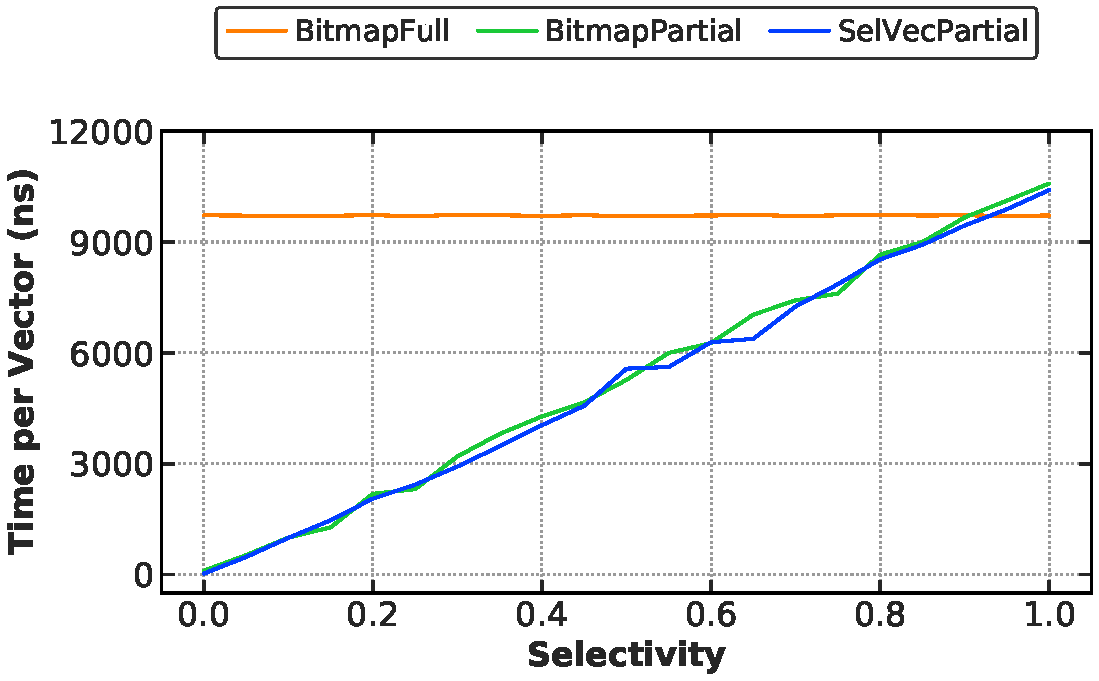
\includegraphics[width=0.9\linewidth]{eval/simple_string_update.pdf}
 \caption{Update operation corresponding to \\ \texttt{\footnotesize WHERE country < `Japan'}}
  \label{fig:varlen_update}
\end{subfigure}
\begin{subfigure}[t]{.49\linewidth}
 \centering
 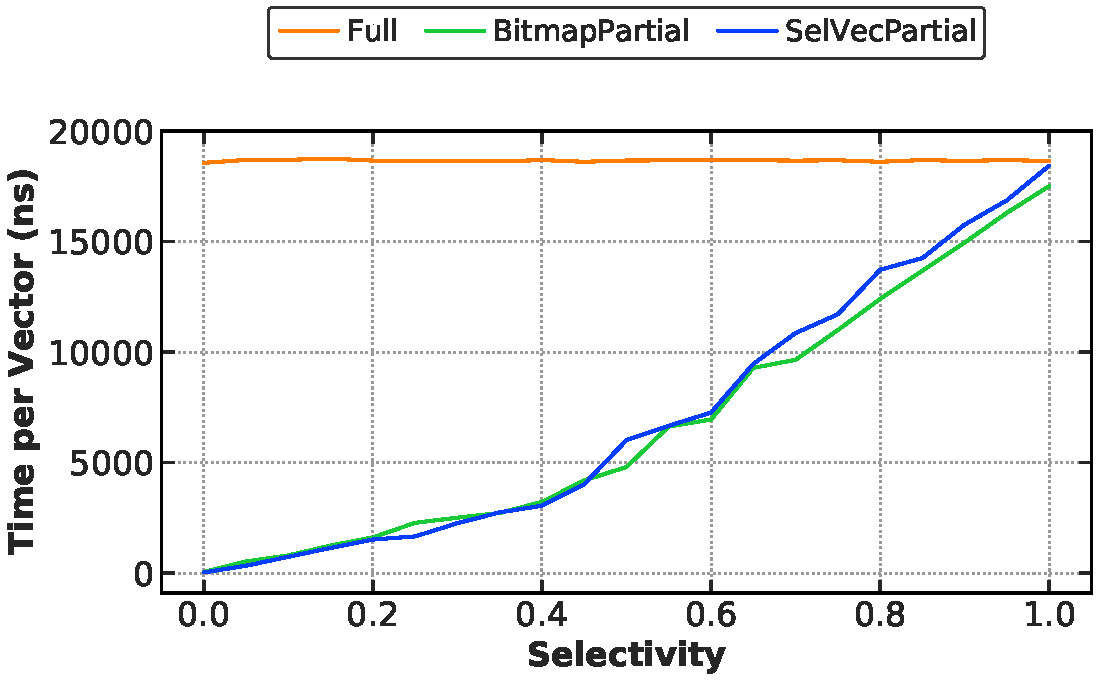
\includegraphics[width=0.9\linewidth]{eval/simple_string_map.pdf}
 \caption{Map operation corresponding to \\ \texttt{\footnotesize SELECT POSITION(`a' in country)}.}
  \label{fig:varlen_map}
\end{subfigure}
\caption{\textbf{Variable Length Data} -- Country names are all short strings that highlight the fact that even cheap variable-length operations should avoid full compute.}
\label{fig:varlen_map_update}
\end{figure}

We first analyze the performance of operations on variable-length data, as is often the case for string operations (e.g., string comparison, sub-string). Let us consider the factors in \cref{fig:perf_equation}. Here, the core operation executes a variable number of instructions depending, for example, on the length of the input strings. As we show in the next experiment, it dominates the iteration logic time, even for short strings. Because data parallelism is not available, the core operation time per tuple is the same across all strategies. The principal factor that differentiates strategies is, therefore, the number of tuples processed, which favors Selective Compute strategies over Full Compute ones.

To confirm this intuition, we run a micro-benchmark using simple string operations on short strings. The Update micro-benchmark performs string comparison, and the Map micro-benchmark performs character location. The strings are all short country names (e.g., USA, Senegal, China). The purpose is to show that the number of tuples processed is the principal performance factor, even for relatively cheap variable-length operations.

The results are shown in \cref{fig:varlen_map_update}. We see that Full Compute (with BitmapFull or Full) consistently performs worst because it processes more tuples, except at full selectivity. At full selectivity, Full Compute and Selective Compute process the same number of tuples, but the former slightly benefits from a simpler iteration logic. We also see that the performance of SelVecPartial is similar to that of BitmapPartial, despite the former's simpler iteration logic, meaning that the core operation is the dominating cost.

The optimal strategy in this scenario is SelVecPartial. It processes fewer tuples than Full Compute strategies and has a slightly cheaper iteration logic than BitmapPartial (though the performance difference is small). Full Compute is only marginally competitive at full selectivity; its benefits are mostly negligible; the more expansive the core operation, the worse Full Compute becomes. 


\subsection{Integer Division}
\begin{figure}[t!]
\captionsetup[subfigure]{justification=justified}
\centering
\begin{subfigure}[t]{.49\linewidth}
 \centering
 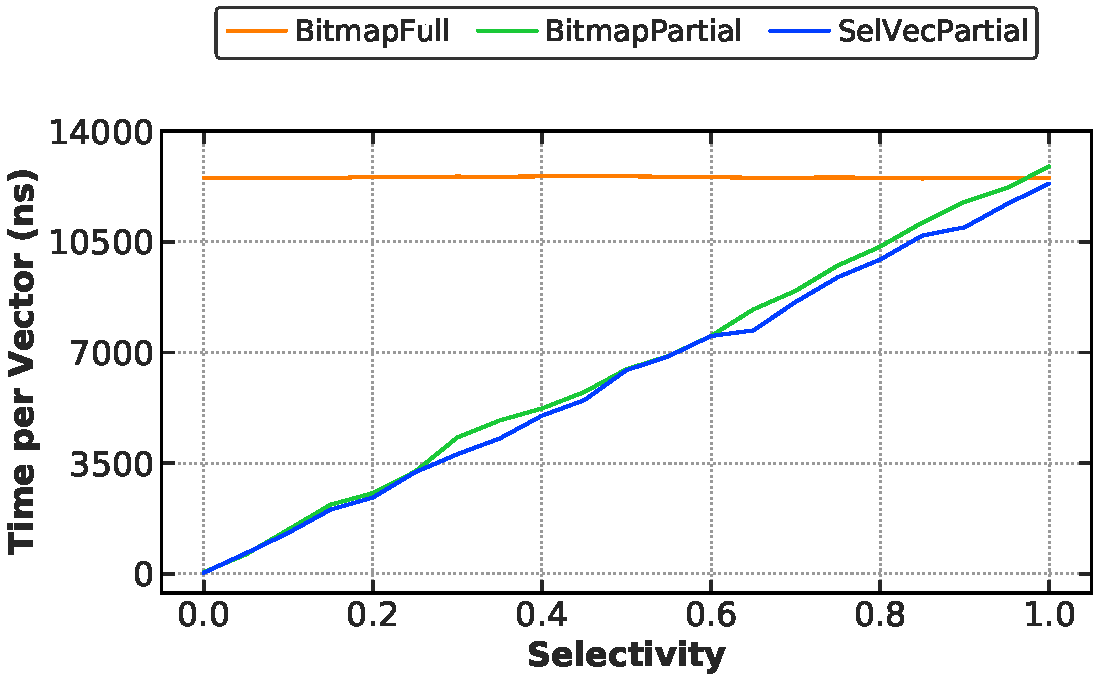
\includegraphics[width=0.9\linewidth]{eval/simple_division_update.pdf}
 \caption{Update operation corresponding to \\ \texttt{\footnotesize WHERE col1 \% col2 < val}.}
  \label{fig:division_update}
\end{subfigure}
\begin{subfigure}[t]{.49\linewidth}
 \centering
 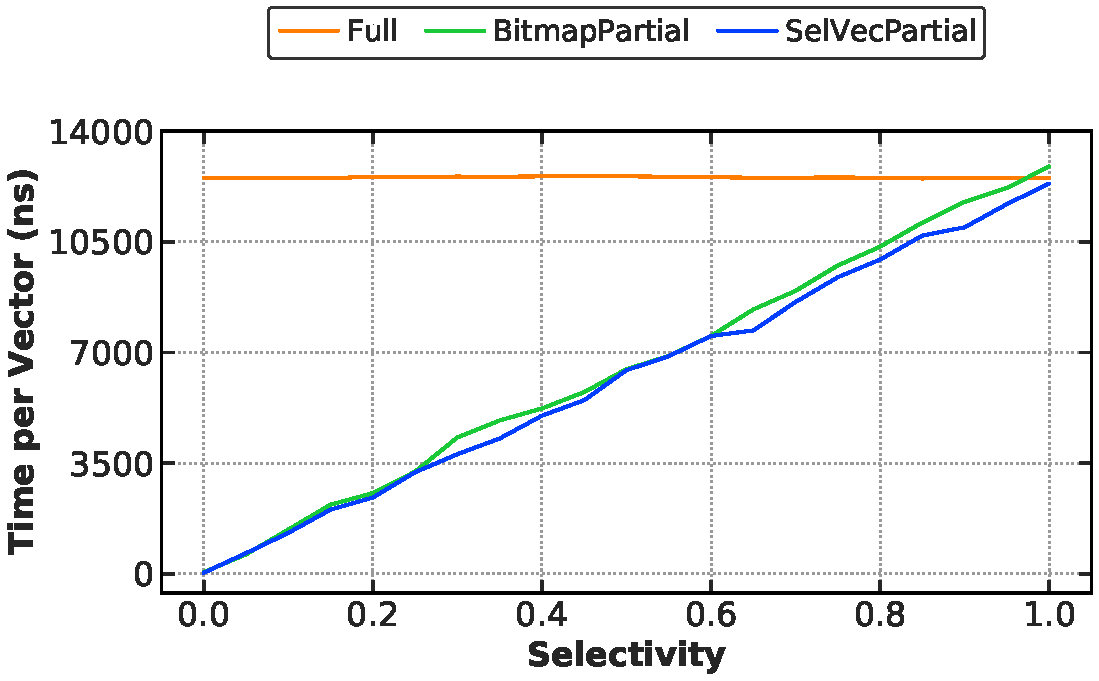
\includegraphics[width=0.9\linewidth]{eval/simple_division_map.pdf}
 \caption{Map operation corresponding to \\ \texttt{\footnotesize SELECT col1 / col2}.}
  \label{fig:division_map}
\end{subfigure}
\caption{\textbf{Integer Division.}}
\label{fig:division_map_update}
\end{figure}
Second, we analyze the integer division instruction as it does not have a SIMD counterpart. Let us consider the factors in \cref{fig:perf_equation}. Integer division is so expansive that the iteration logic time is negligible compared to the core operation time. Because data parallelism is not available, its cost per tuple is the same across all strategies. Once again, the main factor that differentiates strategies is the number of tuples processed, which favors Selective Compute.

The micro-benchmarks of this section evaluate an Update and a Map primitive that both contain an integer division. The results are shown in \cref{fig:division_map_update}. The explanation of its results is similar to \cref{fig:varlen_map_update}'s: the cost of the integer division and the unavailability of data-parallelism make Full Compute inefficient. SelVecPartial is, once again, the optimal strategy, but only has a slight edge over BitmapPartial due to the former's simpler iteration logic.


We conclude that the number of tuples processed in the dominant performance factor for non-data-parallel primitives, making Full Compute impractical. Because of the small impact of iteration logic time, SelVecPartial has a small performance edge over BitmapPartial, but developers can choose either representation without much affecting performance.


\section{Inefficient Data Parallelism}
\label{inefficientsimd}
\begin{figure}[t!]
\centering
\begin{subfigure}[t]{.49\linewidth}
 \centering
 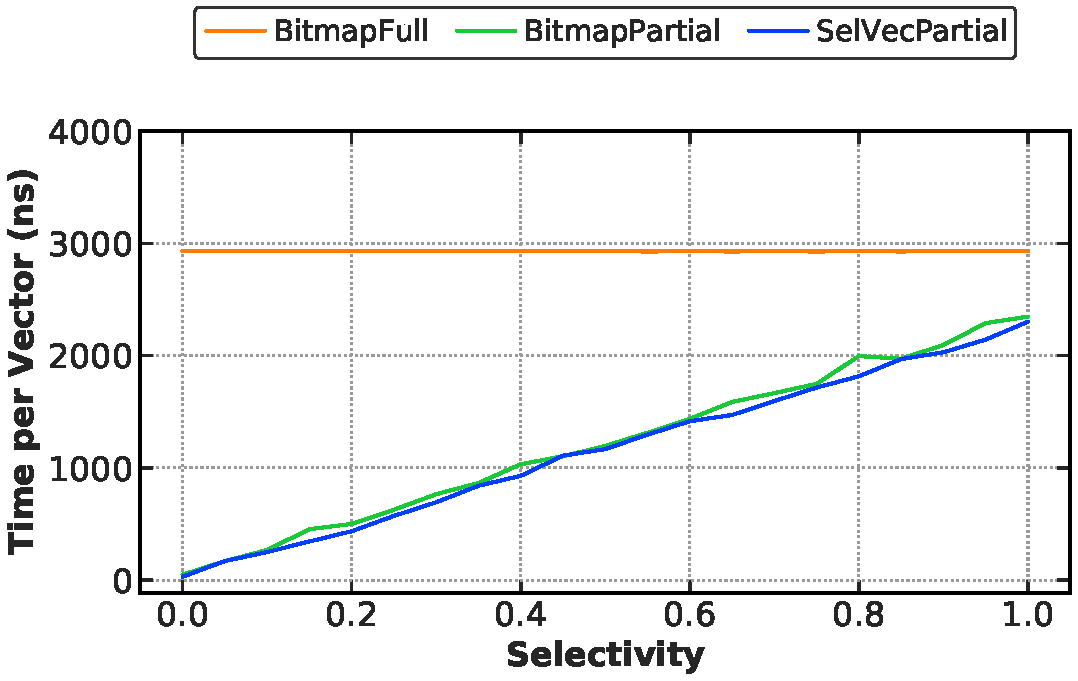
\includegraphics[width=0.9\linewidth]{eval/logical_and_update.pdf}
 \caption{Update operation corresponding to \\ \texttt{\footnotesize WHERE col1 < val1 \&\& col2 < val2}.}
  \label{fig:logical_and_update}
\end{subfigure}%
\begin{subfigure}[t]{.49\linewidth}
 \centering
 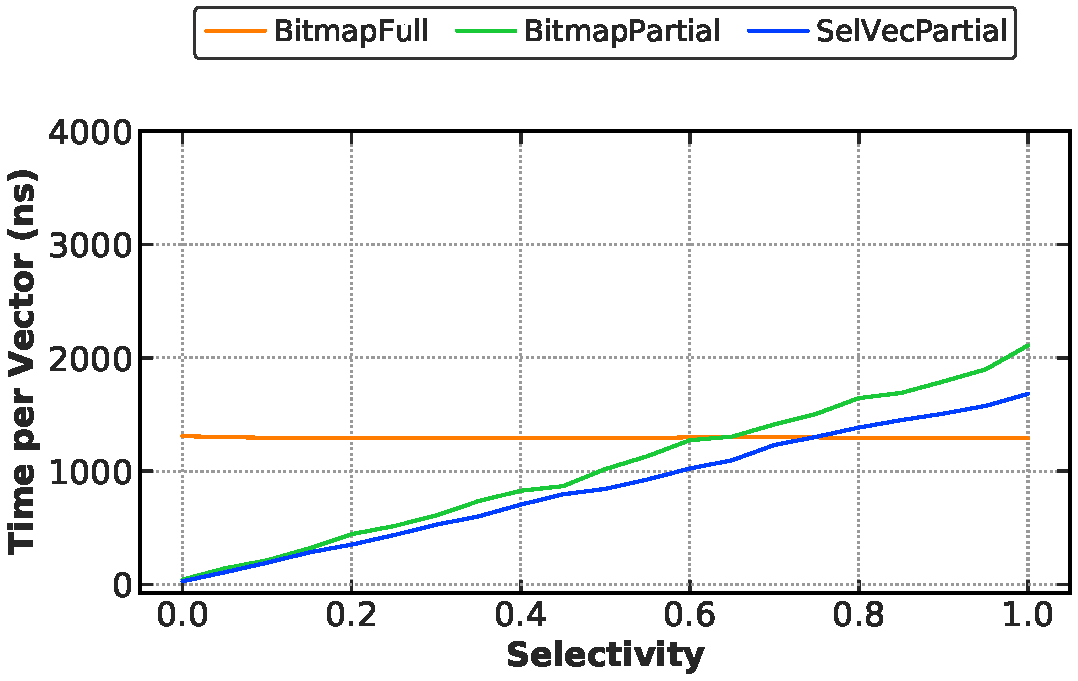
\includegraphics[width=0.9\linewidth]{eval/logical_and_map.pdf}
 \caption{Map operation corresponding to \\ \texttt{\footnotesize SELECT col1 < val1 \&\& col2 < val2}.}
  \label{fig:logical_and_map}
\end{subfigure}
\begin{subfigure}[t]{.49\linewidth}
 \centering
 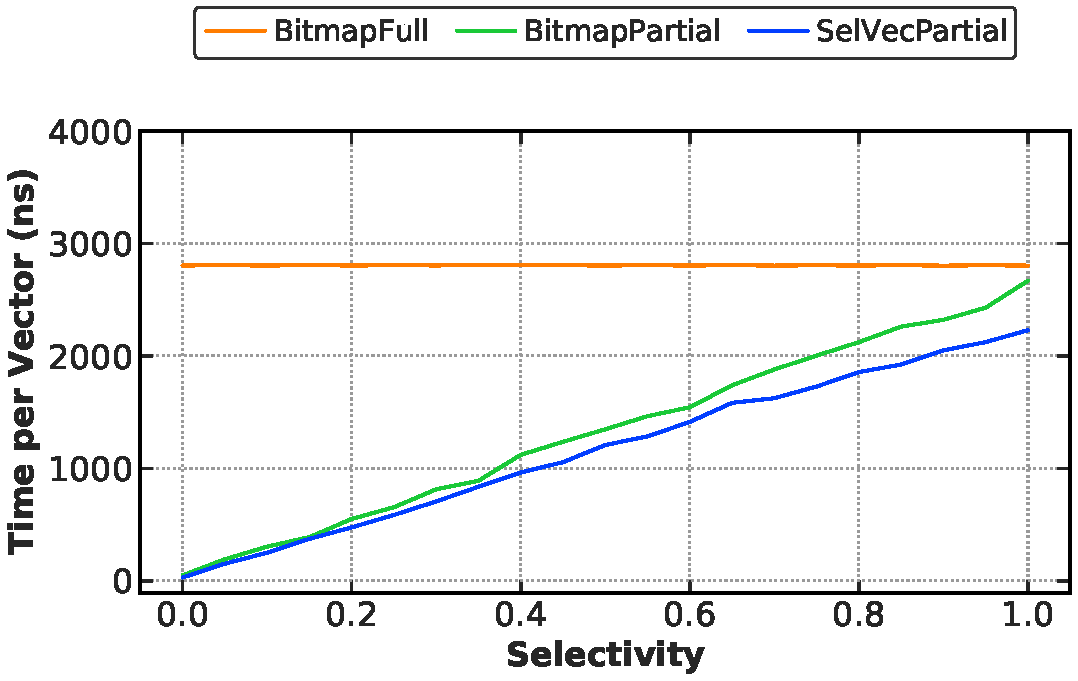
\includegraphics[width=0.9\linewidth]{eval/logical_or_update.pdf}
 \caption{Update operation corresponding to \\ \texttt{\footnotesize WHERE col1 < val1 || col2 < val2}.}
  \label{fig:logical_or_update}
\end{subfigure}%
\begin{subfigure}[t]{.49\linewidth}
 \centering
 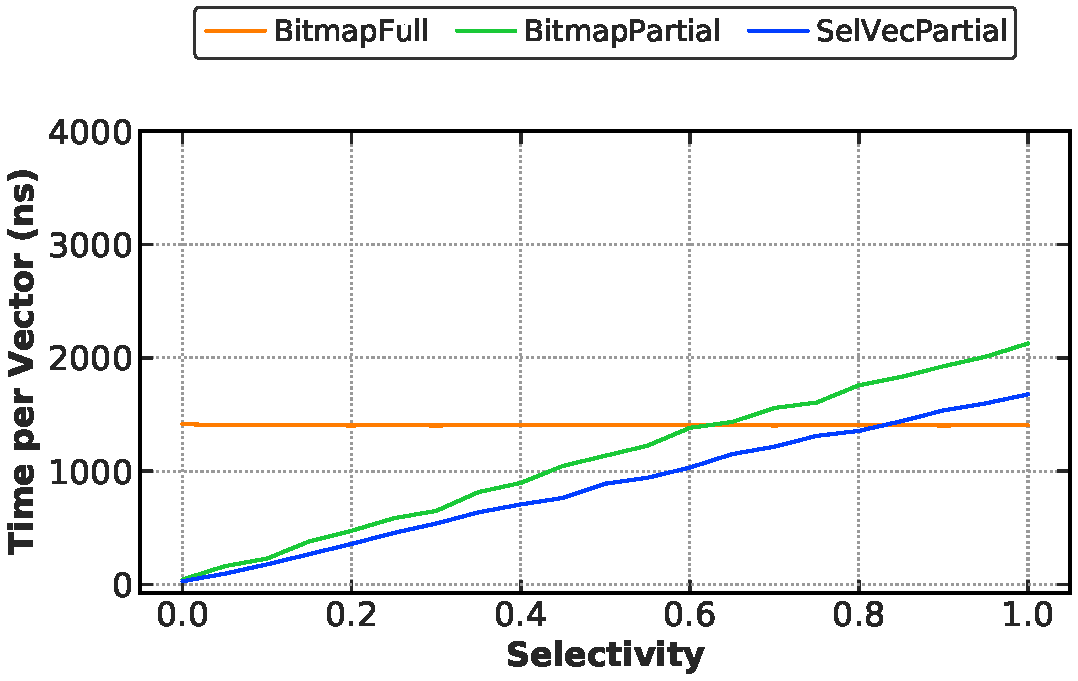
\includegraphics[width=0.9\linewidth]{eval/logical_or_map.pdf}
 \caption{Map operation corresponding to \\ \texttt{\footnotesize SELECT col1 < val1 || col2 < val2}.}
  \label{fig:logical_or_map}
\end{subfigure}

\caption{\textbf{Branching Operations} -- Each operation contains one branch because of boolean short-circuiting.}
\label{fig:logical_map_update}
\end{figure}

\begin{figure}[t!]
\centering
\begin{subfigure}[t]{.49\linewidth}
 \centering
 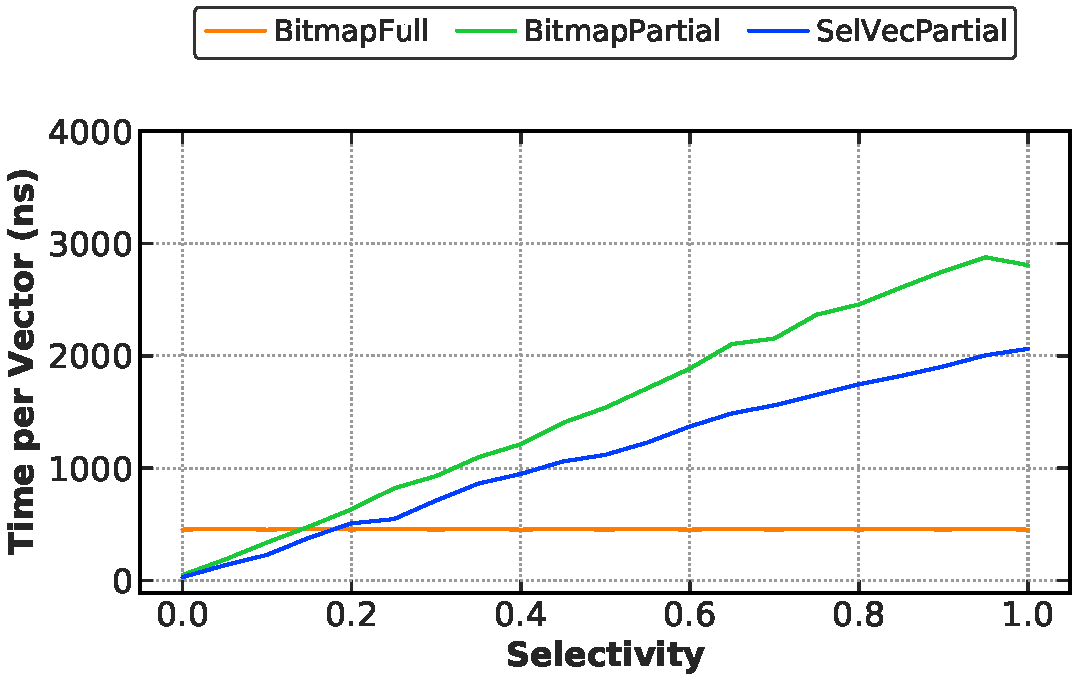
\includegraphics[width=0.9\linewidth]{eval/bitwise_and_update.pdf}
 \caption{Update operation corresponding to \\ \texttt{\footnotesize WHERE col1 < val1 \& col2 < val2}.}
  \label{fig:bitwise_and_update}
\end{subfigure}%
\begin{subfigure}[t]{.49\linewidth}
 \centering
 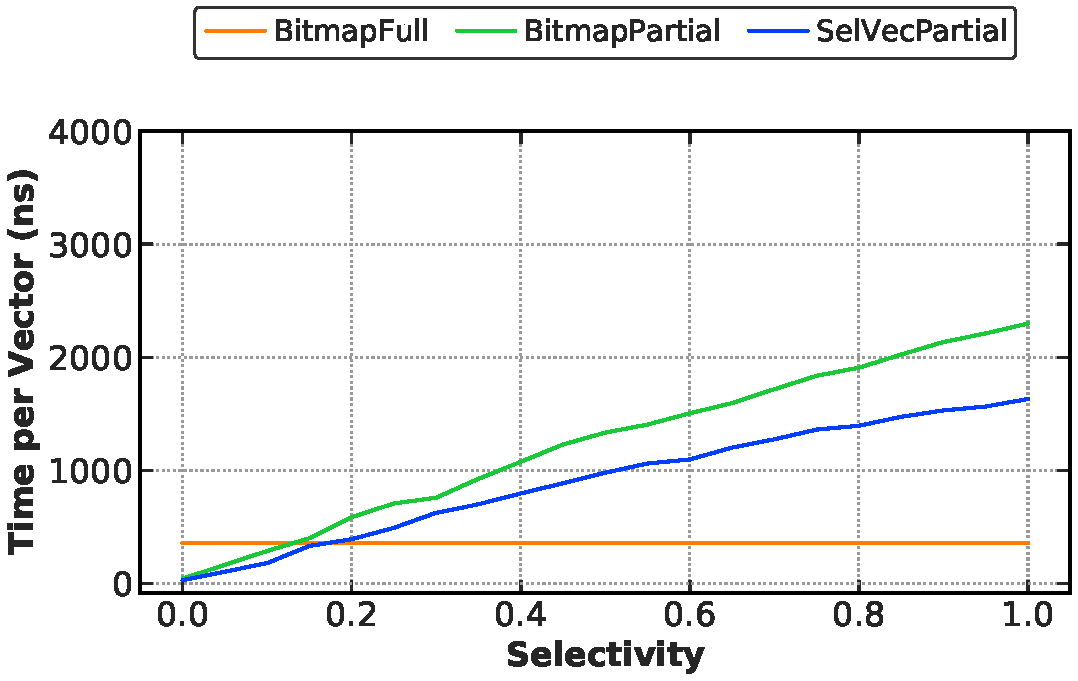
\includegraphics[width=0.9\linewidth]{eval/bitwise_and_map.pdf}
 \caption{Map operation corresponding to \\ \texttt{\footnotesize SELECT col1 < val1 \& col2 < val2}.}
  \label{fig:bitwise_and_map}
\end{subfigure}
\begin{subfigure}[t]{.49\linewidth}
 \centering
 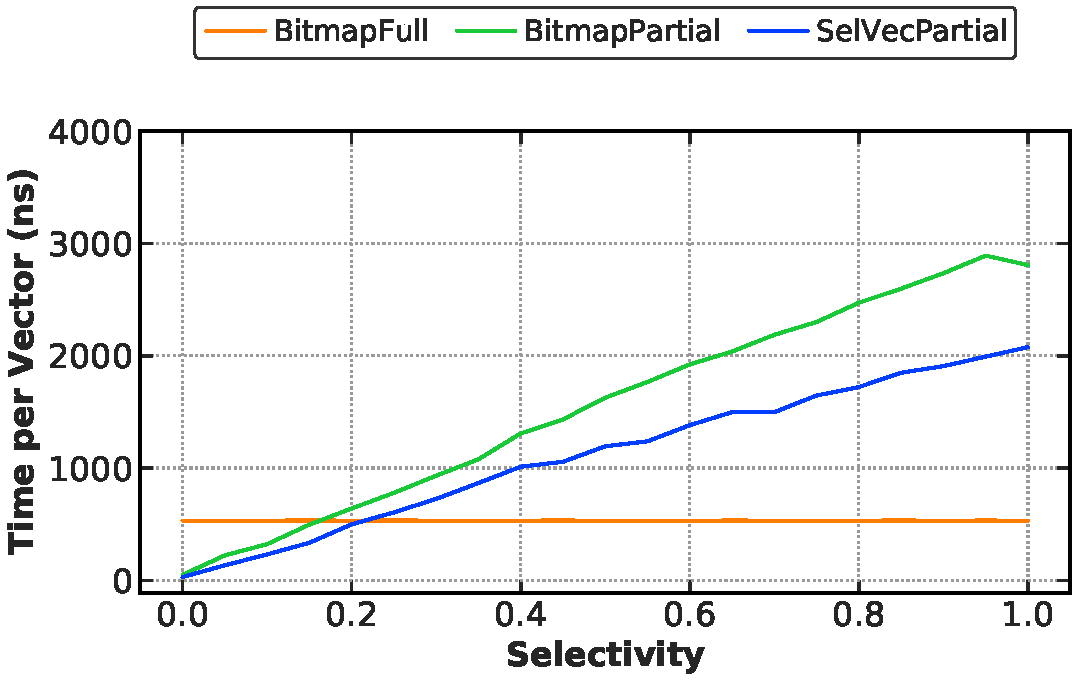
\includegraphics[width=0.9\linewidth]{eval/bitwise_or_update.pdf}
 \caption{Update operation corresponding to \\ \texttt{\footnotesize WHERE col1 < val1 | col2 < val2}.}
  \label{fig:bitwise_or_update}
\end{subfigure}%
\begin{subfigure}[t]{.49\linewidth}
 \centering
 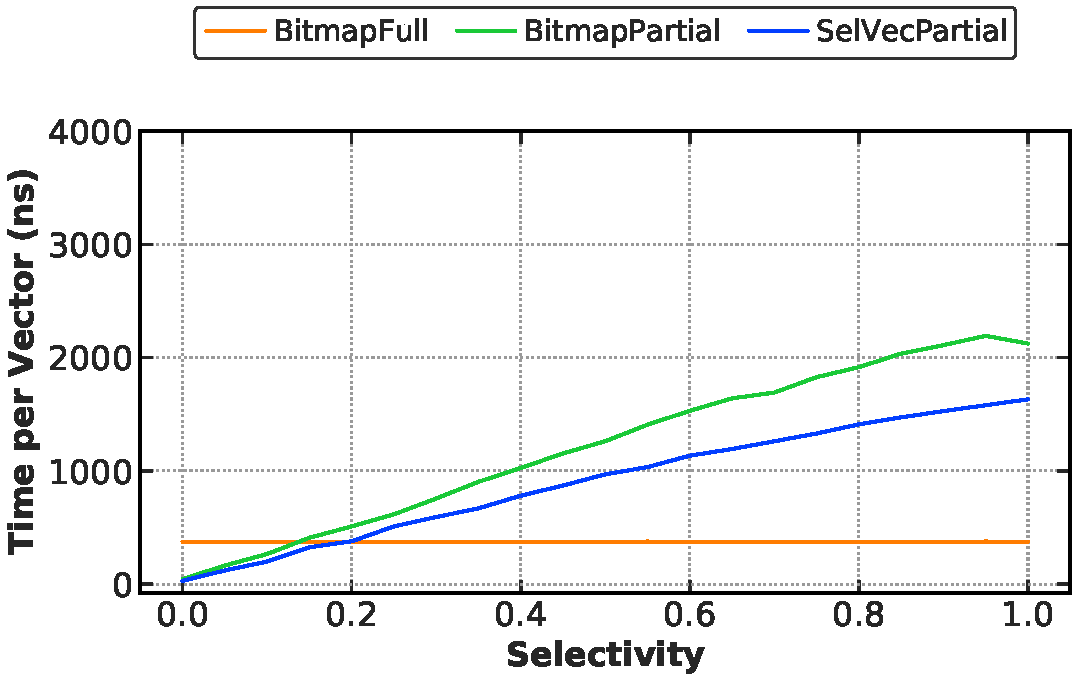
\includegraphics[width=0.9\linewidth]{eval/bitwise_or_map.pdf}
 \caption{Map operation corresponding to \\ \texttt{\footnotesize SELECT col1 < val1 | col2 < val2}.}
  \label{fig:bitwise_or_map}
\end{subfigure}

\caption{\textbf{Bitwise Operations} -- The increase in performance compared to \cref{fig:logical_map_update} is due to the lack of branching.}
\label{fig:bitwise_map_update}
\end{figure}

To study the effect of inefficient use of SIMD instructions, we now consider core operations with branching code. \cref{chapter4} will discuss primitives that contain pointer manipulation and several memory accesses. SIMD strategies (e.g., BitmapFull) benefit from processing multiple tuples at a time, but suffer from executing more code than SISD strategies (e.g., SelVecPartial). Their core operation time per tuple may even decrease depending on the branching structure (e.g., having to execute all branches of a switch statement).  Thus, if Full Compute can outperform Selective Compute at all, it will do so at the highest selectivities because the small reduction in time spent per tuple cannot compensate for the higher number of tuples processed. Among SISD strategies, SelVecPartial will outperform BitmapPartial due to its simple iteration logic.

To determine the impact of a single branch within the core operation, we implemented primitives that perform logical and/or operations. Due to boolean short-circuiting, these primitives will contain exactly one branch. We have confirmed that the compiler manages to auto-vectorize Full Compute strategies. The results are shown in \cref{fig:logical_map_update}. We can see that Full Compute is either always the worst strategy (e.g., in \cref{fig:logical_or_update}), or only competitive at high selectivities ($>= 0.85$ in \cref{fig:logical_or_map}). To confirm that branching is indeed responsible for the poor performance of Full Compute, we implemented branch-less primitives with bitwise and/or operations rather than logical ones. The results are in \cref{fig:bitwise_map_update}. Full Compute now outperforms Selective Compute for selectivities $<= 0.2$, confirming that branching code significantly hurts SIMD strategies' performance.

In conclusion, though Full Compute can sometimes be competitive at the highest selectivities, we recommend, for the sake of simplicity, the SelVecPartial strategy.

\section{Straight-Line and Data-Parallel Core Operations}
\label{sldpsection}

We now consider core operations with Straight-line and data-parallel (SLDP) code, i.e., non-branching code that can efficiently leverage SIMD instructions. Primitives that only perform arithmetic (without integer division) and bitwise instructions fall under this category. Let us consider the equation in \cref{prim_perf_section} to analyze the performance of each strategy in this scenario. Full Compute strategies (e.g., BitmapFull, Full) can leverage SIMD instructions to significantly reduce the iteration logic and core operation time per tuple. AVX512 \cite{intel2019} integer addition instructions, for example, performs 8 parallel 64-bit additions in a single cycle. We, therefore, expect Selective Compute strategies to only be competitive when the selectivity is very low, meaning that Full Compute processes far more tuples. SelVecManual is the exception: it is a Selective Compute strategy that uses SIMD instructions. Its gain in iteration logic time is, however, not as high as that of Full Compute strategies because it uses a \texttt{gather} instruction \cite{intel2019} to collect the elements at the selected indices (shown in \cref{fig:rationale_selvec}). The higher the core operations time per tuple, the less important the \texttt{gather} overhead because iteration logic time becomes more and more insignificant. Thus, we expect SelVecManual to be competitive with Full Compute at medium or below selectivities depending on the core operation. The next experiments will quantify the differences between each strategy.

\begin{figure}[t!]
    \centering
    \makebox[\textwidth]{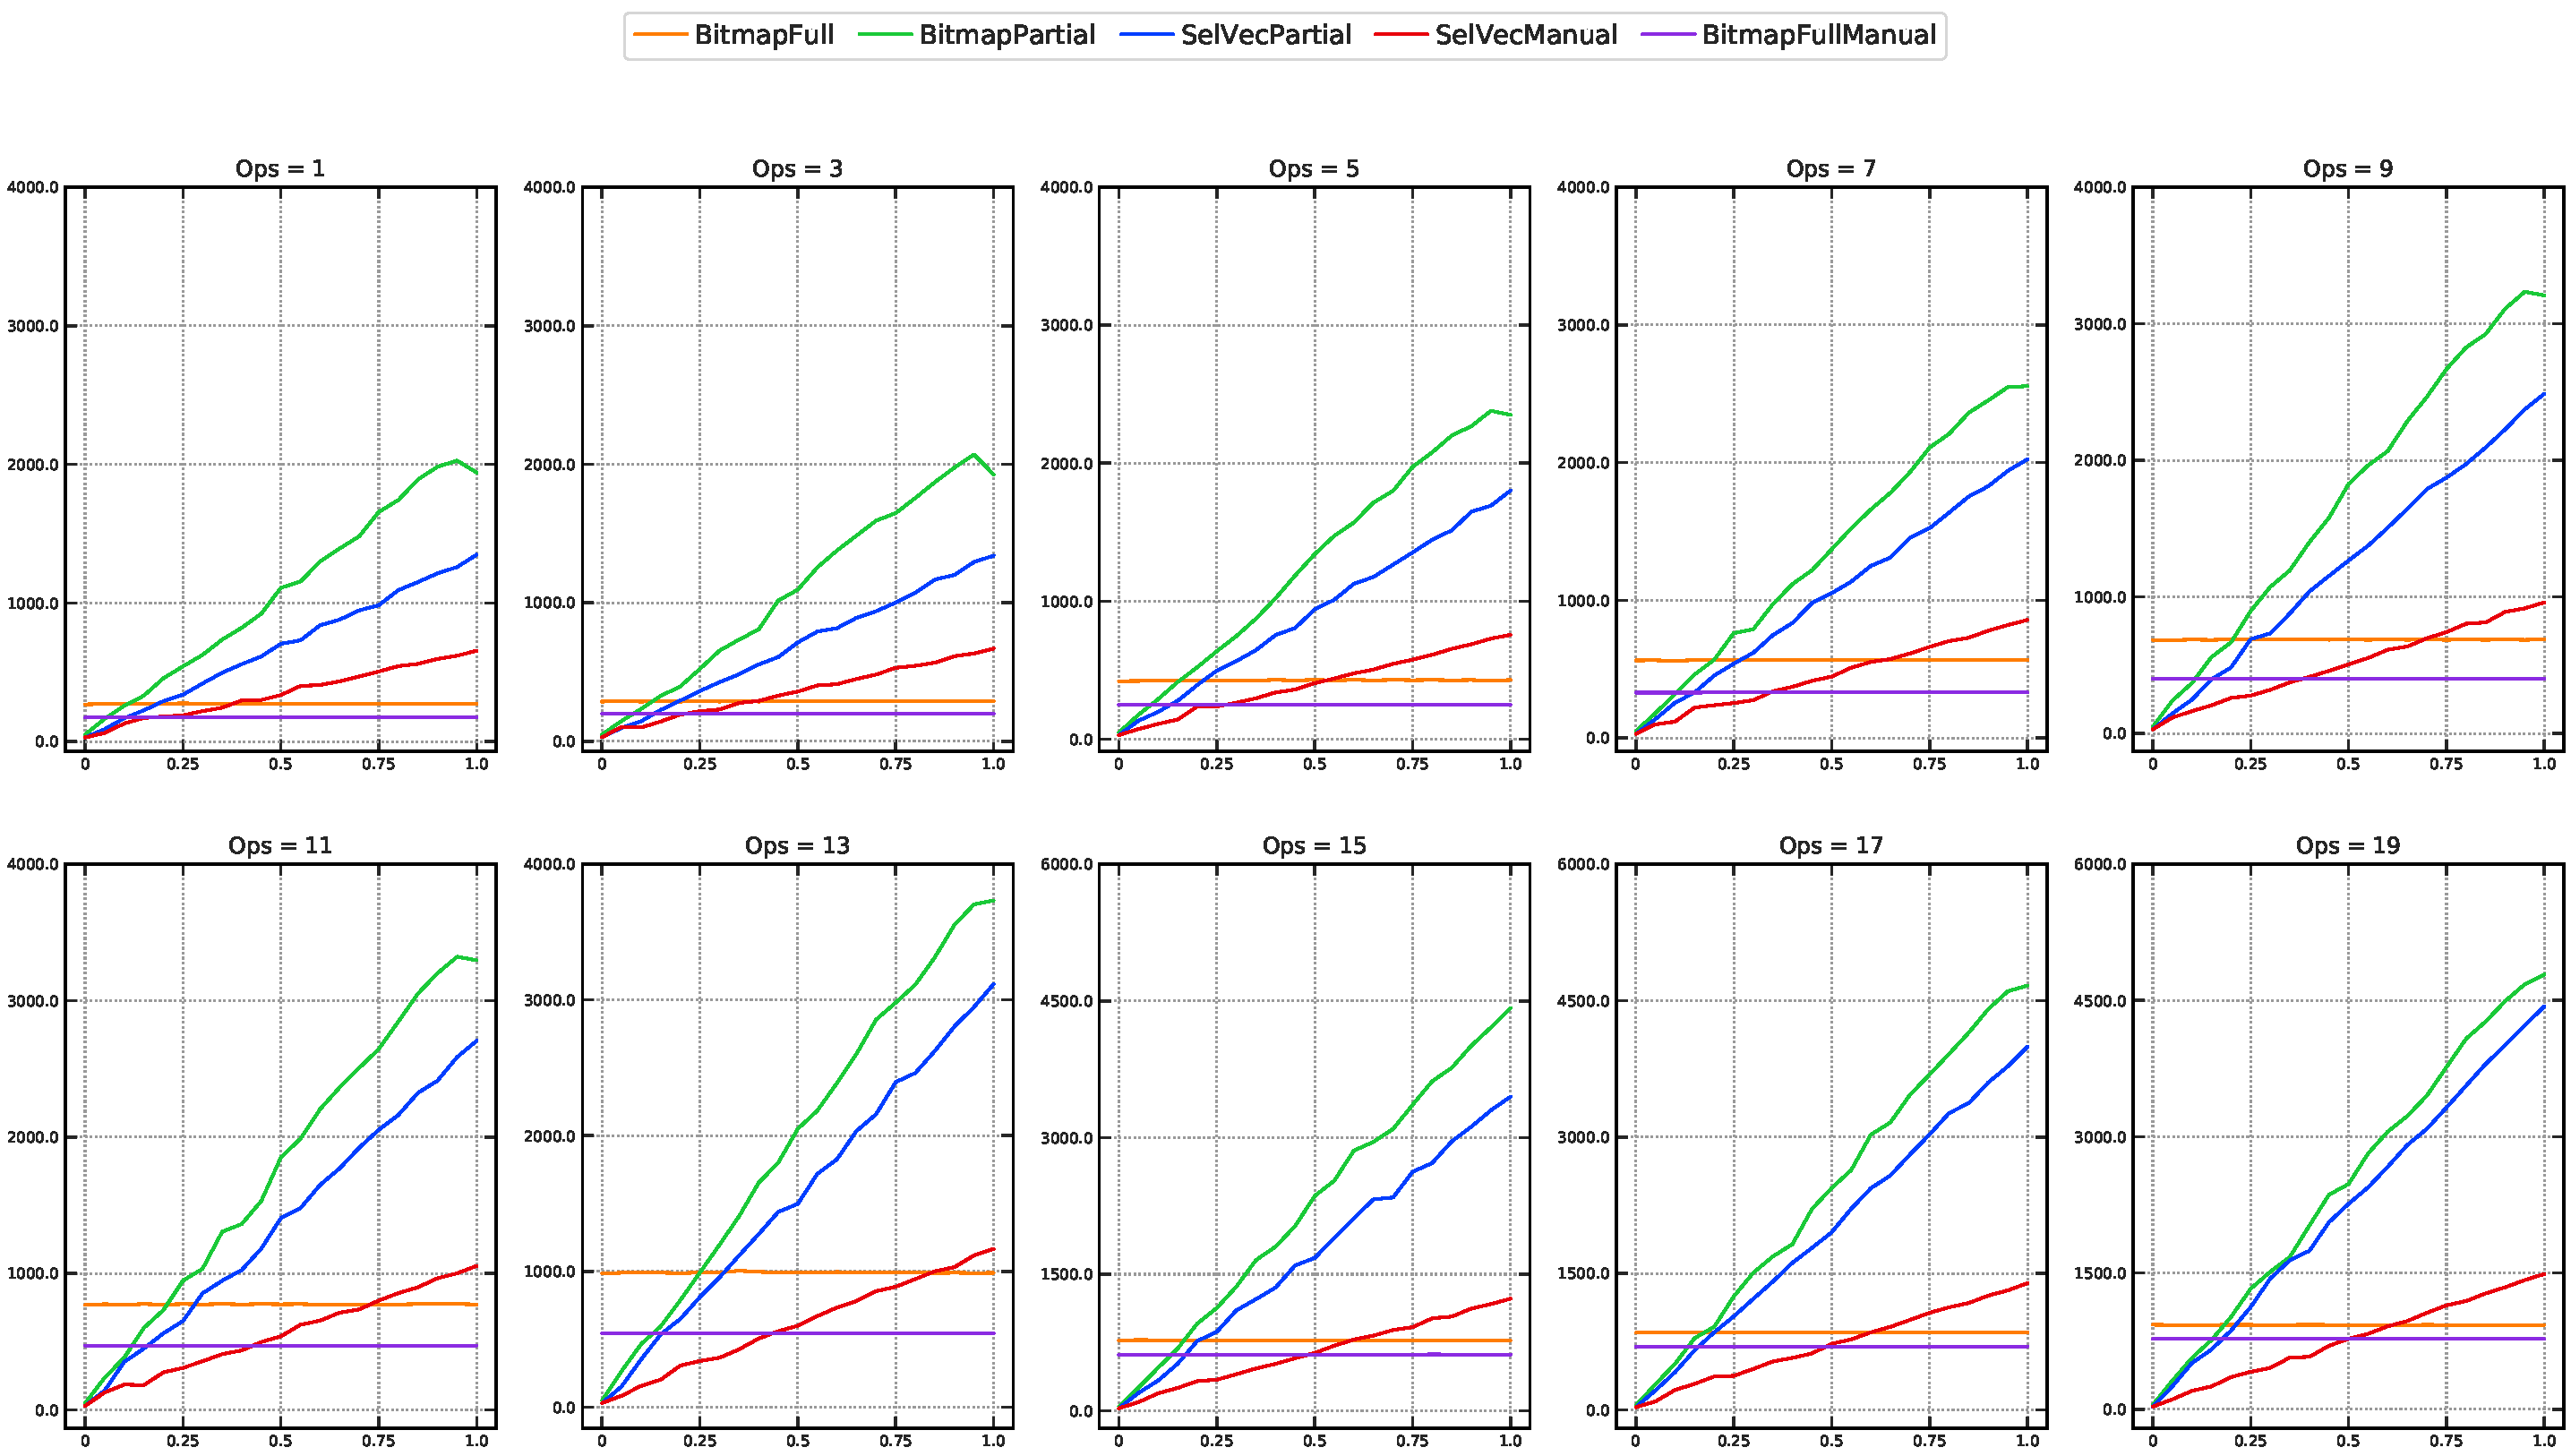
\includegraphics[width=.9\paperwidth]{eval/snbs_update.pdf}}
    \caption{\textbf{SNBS Update Operations} -- For Updates, SelVecManual relies on the \texttt{compress\_store} SIMD instruction rather than on \texttt{scatter}, which reduces its overhead.}
    \label{fig:snbs_update}
\end{figure}

\begin{figure}[t!]
    \centering
    \makebox[\textwidth]{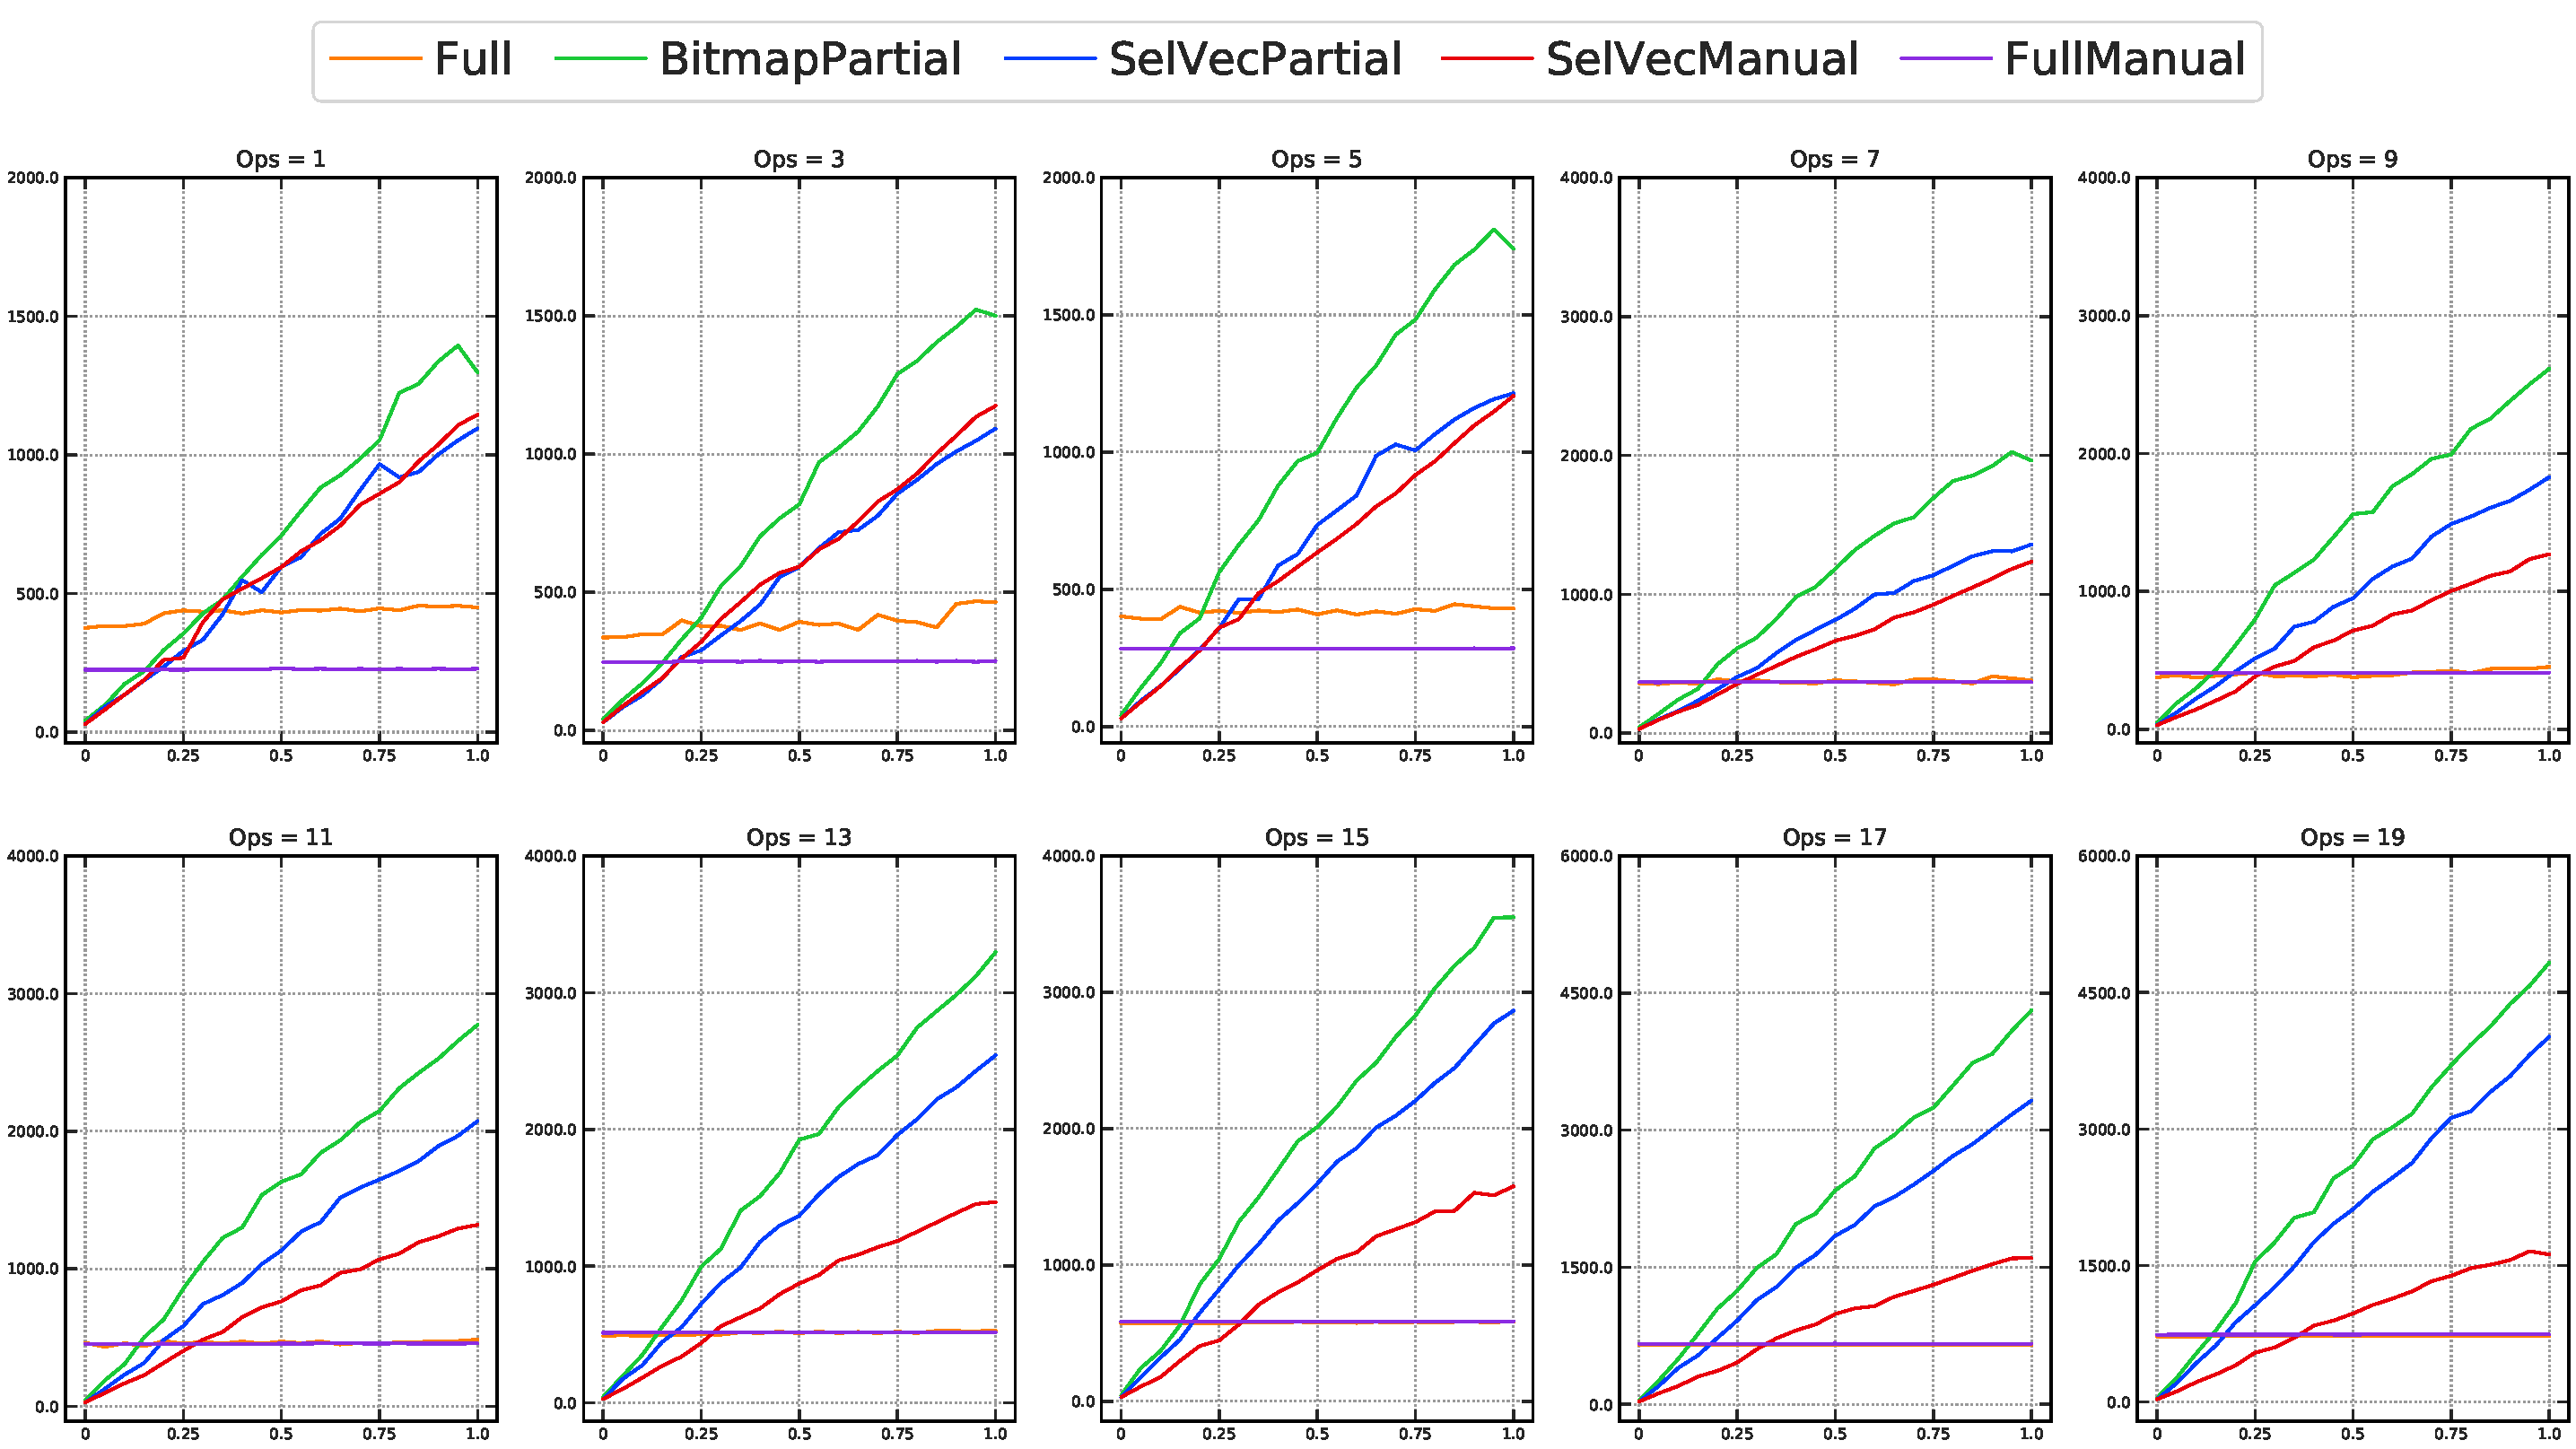
\includegraphics[width=.9\paperwidth]{eval/snbs_map.pdf}}
    \caption{\textbf{SNBS Map Operations} -- For Maps, SelVecManual relies on the \texttt{scatter} SIMD instruction, which explains why it initially does not perform better than SelVecPartial.}
    \label{fig:snbs_map}
\end{figure}

\begin{figure}[t!]
\captionsetup[subfigure]{justification=justified}
\centering
\begin{subfigure}[t]{.49\linewidth}
 \centering
 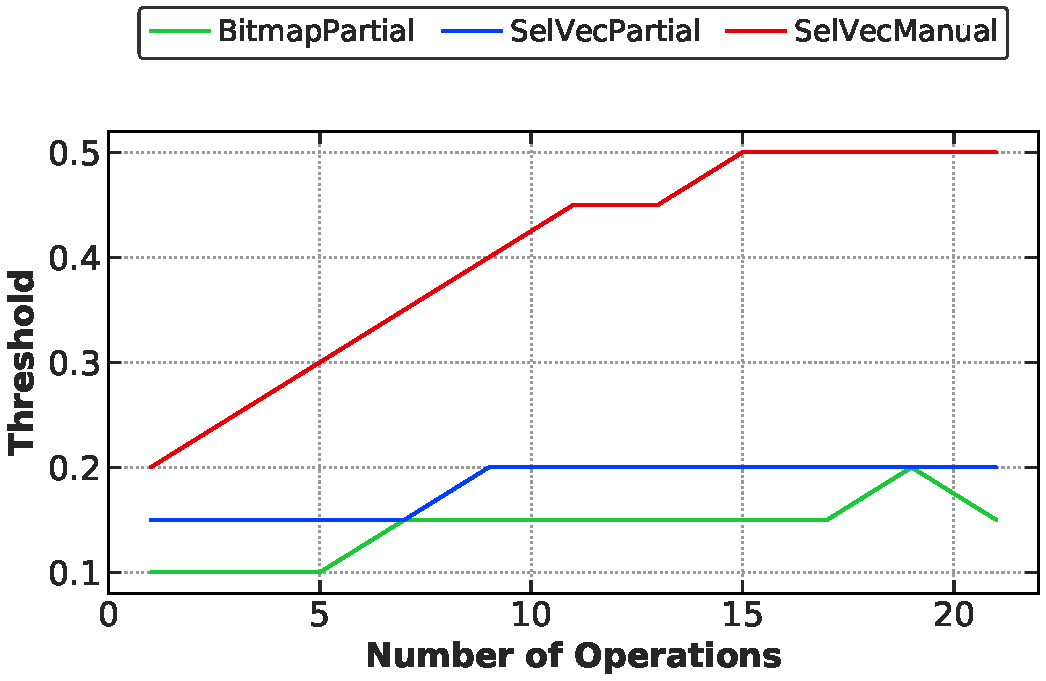
\includegraphics[width=0.9\linewidth]{eval/snbs_thres_update.pdf}
 \caption{Update thresholds between BitmapFullManual and Selective Compute strategies.}.
  \label{fig:snbs_thres_update}
\end{subfigure}
\begin{subfigure}[t]{.49\linewidth}
 \centering
 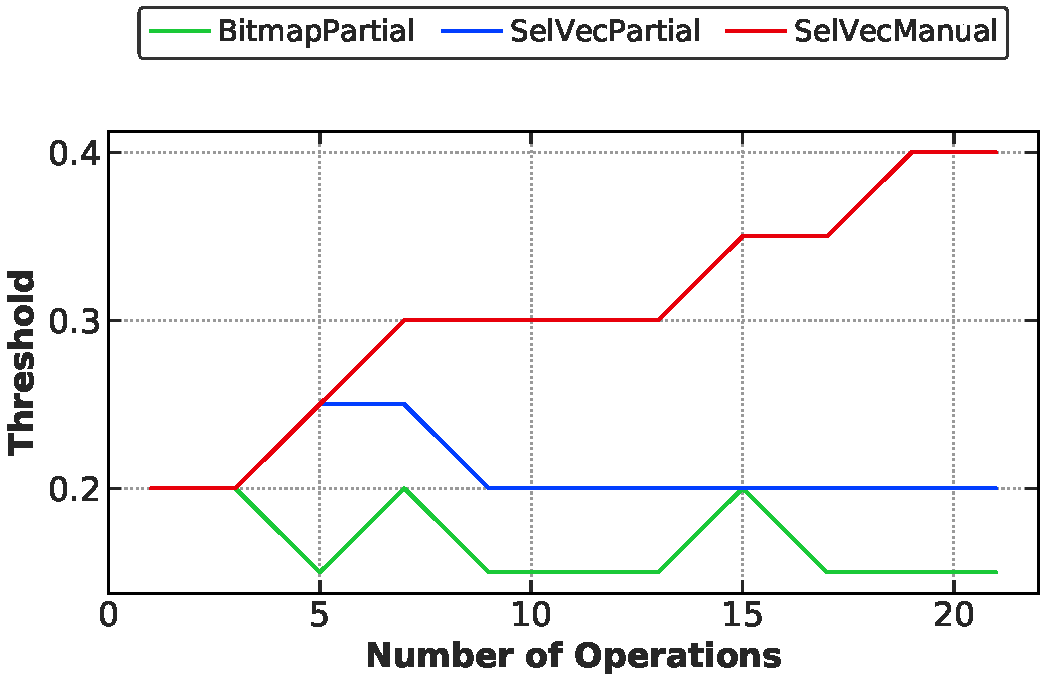
\includegraphics[width=0.9\linewidth]{eval/snbs_thres_map.pdf}
 \caption{Map thresholds between FullManual and Selective Compute strategies.}
  \label{fig:snbs_thres_map}
\end{subfigure}
\caption{\textbf{Mixed Compute Thresholds} -- The Full Compute strategies are BitmapFullManual and FullManual because compiler auto-vectorization does not consistently use AVX512 registers.}
\label{fig:snbs_thres}
\end{figure}


We implemented Update and Map primitives in which the core operation contains single-cycle arithmetic and bitwise instructions. We progressively increase the number of such instructions to increase the core operations time per tuple and quantify the selectivity thresholds above which Full Compute strategies become faster than Selective Compute ones. The results are shown in \cref{fig:snbs_update,fig:snbs_map} (for Updates and Maps). The selectivity thresholds for each graph are respectively in \cref{fig:snbs_thres_update,fig:snbs_thres_map}. Let us analyze the results in detail:
\begin{itemize}
    \item In all experiments, SelVecPartial performs better than BitmapPartial. As explained in the previous chapter, this is only due to a simpler iteration logic.
    \item SelVecManual is always the best Selective Compute strategy because it uses data-parallelism to reduce the time spent per tuple.
    \item Manual Vectorization (with FullManual and BitmapFullManual) sometimes performs much better than Auto-Vectorization (with Full and BitmapFull). For example, in \cref{fig:snbs_update}'s graph for \texttt{NumOps=13}, BitmapFullManual is $1.8$ times faster than BitmapFull. With further investigation of the generated code, we discovered that the compiler is overly conservative when it comes to using AVX512. AVX512 registers result in decreased CPU frequency \cite{avx512_registers}, so the compiler is careful not always to use them. It often uses AVX2 registers instead. We, on the other hand, always use AVX512.
    \item The thresholds for SelVecPartial and BitmapPartial, shown in \cref{fig:snbs_thres_update,fig:snbs_thres_map}, prove that these strategies are only competitive with Full Compute at low selectivities ($<= 0.2$) because, as explained above, they do not use SIMD instructions.
    \item The threshold for SelVecManual, on the other hand, increases with the number of operations because its iteration logic overhead becomes more and more insignificant as the core operation time increases. SelVecManual thus benefits from data-parallelism while processing fewer tuples than Full Compute strategies. The iteration logic difference is never entirely negligible, though; the threshold is medium at best ($0.5$ at 15 operations in \cref{fig:snbs_thres_update}). 
\end{itemize}



This analysis shows the importance of Mixed Compute: we should use Selective Compute below the selectivity thresholds, and Full Compute otherwise. The next section details our implementation of Mixed Compute.

\section{Implementing Mixed Compute}
\label{mixedcompute}
The previous section showed that for a given SLDP primitive, there is a threshold below which SelVecManual is optimal and above which BitmapFullManual and FullManual are optimal for Updates and Maps respectively. To find this threshold, we can run a micro-benchmark similar to the one in \cref{fig:snbs_thres}. The lowest selectivity at which the runtime of Full Compute strategies exceeds that of Selective Compute strategies represents the Mixed Compute threshold for a given primitive. In summary, the optimal SLDP strategy is as follows:
\begin{itemize}
\item For Maps: Full or FullManual when the selectivity is above the threshold, and SelVecManual when the selectivity is below the threshold.
\item For Updates: BitmapFull or BitmapFullManual when the selectivity is above the threshold, and SelVecManual when the selectivity is below the threshold. Note that the BitmapFull and SelVecManual have different filter representations.  There is a small cost associated with the conversion from Bitmap to SelVec, but, in practice, other operations always follow an update (e.g., there is a projection after a scan filter). The subsequent operations often amortize the conversion cost. For small queries, in which the amortization does not neutralize the conversion cost, BitmapPartial can slightly outperform SelVecManual because it maintains the Bitmap representation. Nonetheless, as we show in \cref{chapter4}, its gains are mostly negligible.
\end{itemize}

\section{Vectorization Decision Tree}
\begin{figure}[t!]
    \centering
    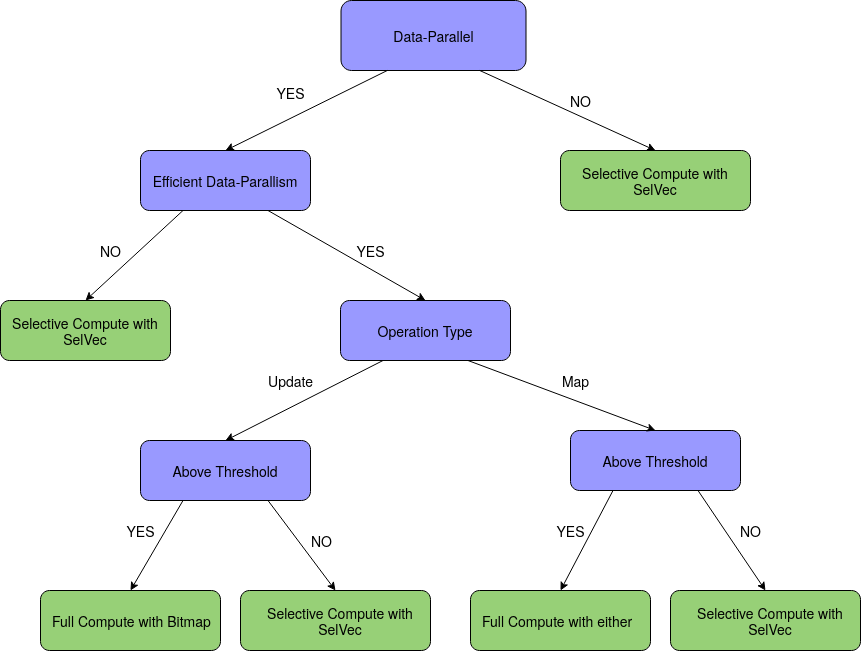
\includegraphics[scale=0.5]{images/DecisionTree.png}
    \caption{\textbf{The Summary Decision Tree} -- It summarizes the results in this chapter.}
    \label{fig:filter_decision_tree}
\end{figure}

The decision tree in \cref{fig:filter_decision_tree} summarizes the results of this chapter. It uses the experiments above to derive the optimal implementation strategy depending on the core operation and the input selectivity of a given primitive. The \textbf{Data-Parallel} node, the \textbf{Effecient Data-Parallelism} respectively use the results in \cref{nondataparallel} and \cref{inefficientsimd} that designated SelVecPartial as the optimal strategy. The \textbf{Operation Type} and \textbf{Above Threshold} nodes use the results in \cref{sldpsection} and \cref{mixedcompute} that designed a Mixed Compute strategies for each primitive type (Update or Map).


The tree assumes that the system developer implements all representations and compute strategies. The total number of variants of each primitive will be extensive, which constitutes a costly engineering endeavor. To remedy this cost, we note that the BitmapPartial strategy does not perform significantly worse than SelVecPartial or SelVecManual at most selectivities. Developers can, thus, focus on focus on the Bitmap representation without losing too much performance. Switching between Full and Selective Compute is critical, though; the performance gain is too significant.

\chapter{Experimental Evaluation}
\label{chapter4}

We now evaluate the benefits of the decision tree in \cref{chapter3}. For this evaluation, we implemented the strategies for a subset of queries from the TPCH benchmark, a decision support system workload that simulates an OLAP environment~\cite{tpch}. We use a scale factor of 10 ($\sim$10~GB). The hardware setup is unchanged from the previous chapter. We use the columnar storage engine of the NoisePage DBMS \cite{noise_page}. The string columns are all dictionary compressed for faster processing \cite{abadicompression}. Whenever the compiler (clang \cite{clang}) failed to SIMD vectorize a primitive that should be data-parallel or used AVX2 instead of AVX512, we hand-wrote SIMD code using AVX512 intrinsics \cite{intel2019}.

Each query contains primitive with side-effects (e.g., hash table insertion), and primitives without side-effects (e.g., multiplication of two columns). Given that this thesis focuses on side-effect-free primitives, we report two metrics for each query: the running time of the whole query and the running time of the side-effect free primitives within the query. The output of each query is materialized in memory and printed to the standard output; no network transfer occurs.

\section{Q1: High Selectivity SLDP primitives}
\begin{figure}[t!]
    \centering
    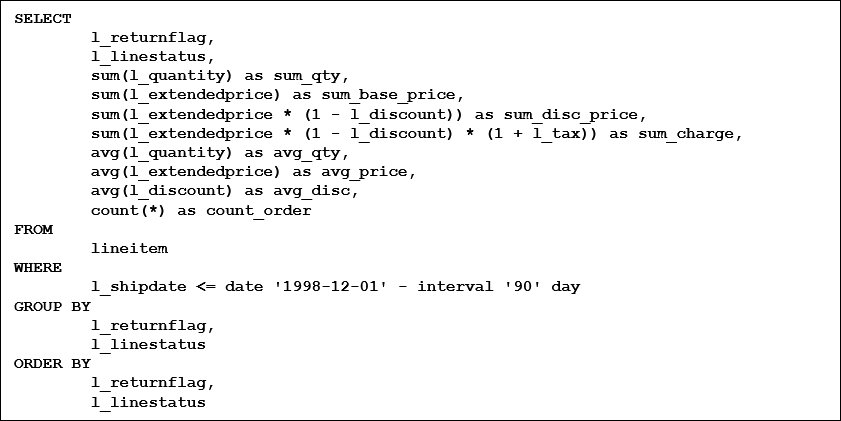
\includegraphics[scale=0.5]{images/TPCH-Q1.png}
    \caption{\textbf{The TPCH Q1 query.}}
    \label{fig:tpch_q1}
\end{figure}

\label{q1section}
\begin{figure}[t!]
\centering
\hspace*{\fill}% 
\begin{subfigure}[t]{.8\linewidth}
 \centering
 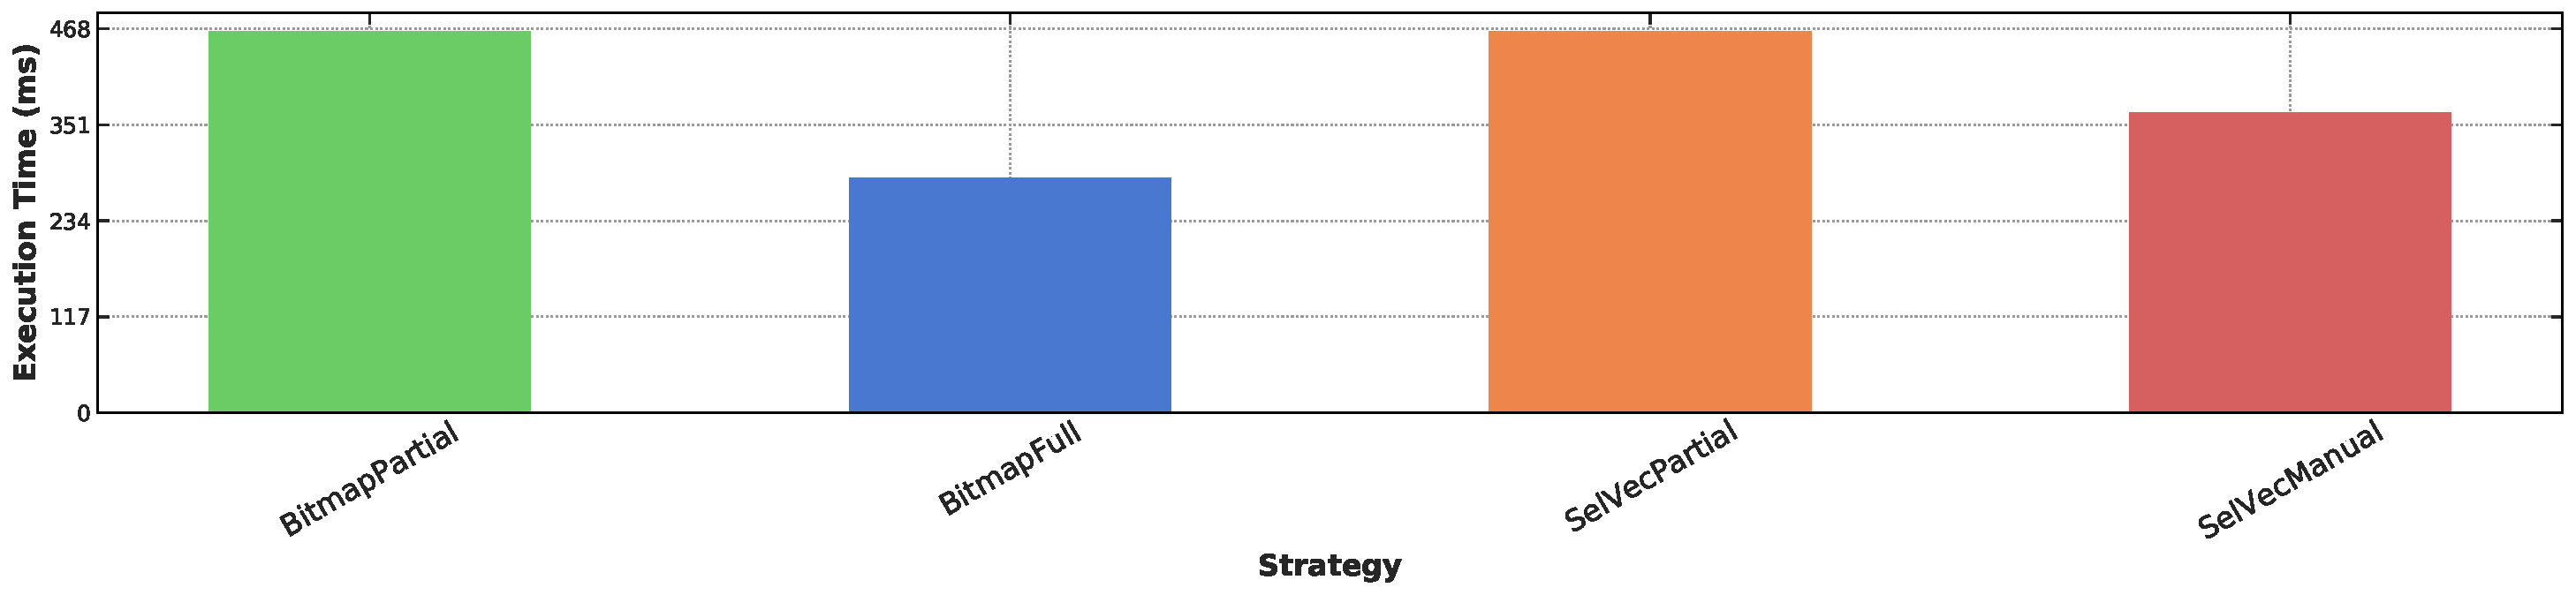
\includegraphics[width=0.9\linewidth]{eval/q1_optimized.pdf}
 \caption{Running time of side-effect free primitives.} \label{fig:q1_optimized}
\end{subfigure}
\hspace*{\fill}%
\vspace*{8pt}%

\hspace*{\fill}%

\begin{subfigure}[t]{.8\linewidth}
 \centering
 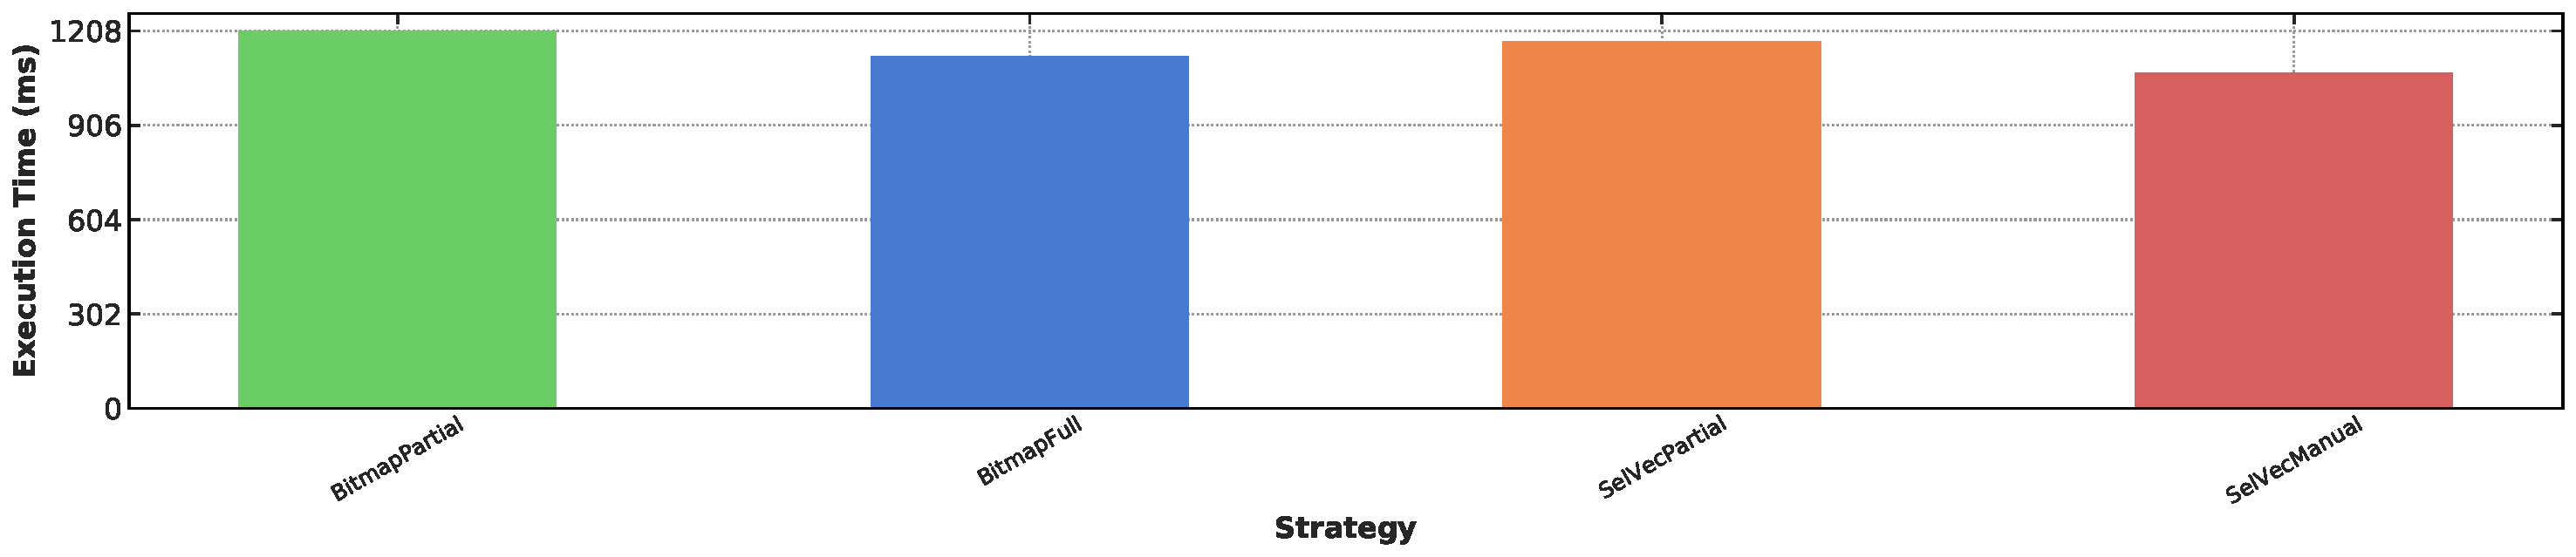
\includegraphics[width=0.9\linewidth]{eval/q1_bench.pdf}
 \caption{Total running time.}
  \label{fig:q1_bench}
\end{subfigure}%
\caption{\textbf{Q1 Performance}}
\label{fig:q1_perf}
\end{figure}

\cref{fig:tpch_q1} shows the SQL code of the Q1 query. It contains a single SLDP filter in its \texttt{WHERE} clause; its selectivity is consistently above $0.95$ for the vectors from the \texttt{lineitem} table. Its \texttt{SELECT} clause contains multiple arithmetic SLDP operations followed by side-effect-full aggregation and order-by operators that dominate the running time. Before the aggregation, there is an SLDP primitive that hashes the \texttt{GROUP BY} keys. Because the selectivity is high and the query is SLDP-heavy, our decision tree favors SIMD vectorized Full Compute strategies. Besides, switching between strategies is not required.

The results for the strategies we implemented are shown in \cref{fig:q1_perf}. We omit the Mixed strategies' measurements because no switching ever occurs in the query plan; they have the same running times as BitmapFull. \cref{fig:q1_optimized} shows the running time of the primitives we optimized. As predicted by our decision tree, the SIMD Full Compute strategy, BitmapFull, best optimizes these primitives. It outperforms BitmapPartial and SelVecPartial (which have SISD primitives) by $1.6\times$, and SelVecManual (which has manually written SIMD primitives) by $1.3\times$. 

The total running times (\cref{fig:q1_bench}) are mostly the same for all queries for two reasons. First, the side-effect-full aggregation, which we do not try to optimize, is the query's dominant component. Second, Intel's implementation of AVX512 instructions decreased CPU speed. This effect explains why clang limits their usage to avoid performance degradations \cite{avx512_registers}. Compare, for example, the BitmapPartial and BitmapFull strategies. They both have the same code for the side-effect-full primitives, but BitmapFull performs them in $838\text{ms}$, whereas BitmapPartial performs them in $739\text{ms}$. Naively avoiding AVX512 instructions is not the solution; AVX2 uses vectors that have half the width of AVX512's, which slows down the execution of SLDP primitives. Careful analysis is thus required to balance the benefits and disadvantages of AVX512 instructions. This analysis is left as future work.


\section{Q6: Mixed Selectivity SLDP Primitives}
\label{q6section}
\begin{figure}[t!]
    \centering
    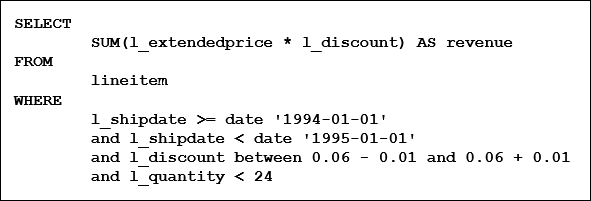
\includegraphics[scale=0.5]{images/TPCH-Q6.png}
    \caption{\textbf{The TPCH Q6 query.}}
    \label{fig:tpch_q6}
\end{figure}
 
\begin{figure}[t!]
\centering
\hspace*{\fill}% 
\begin{subfigure}[t]{.8\linewidth}
 \centering
 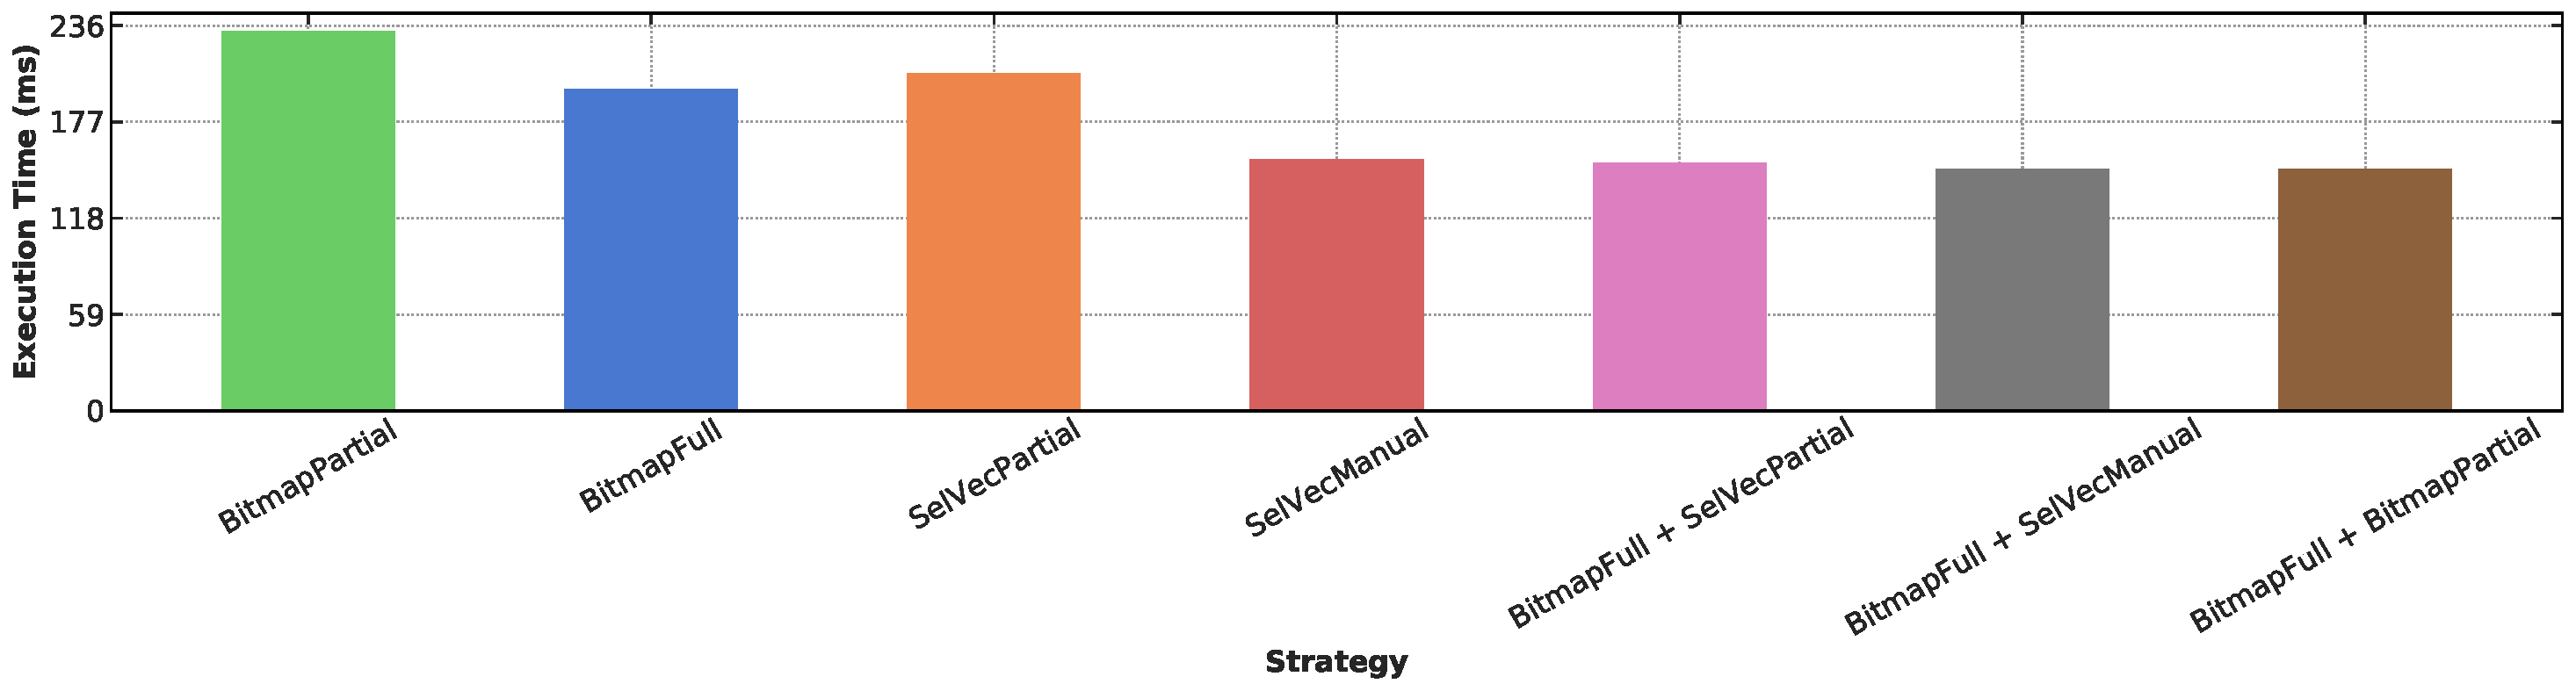
\includegraphics[width=0.9\linewidth]{eval/q6_optimized.pdf}
 \caption{Running time of side-effect free primitives.}
  \label{fig:q6_optimized}
\end{subfigure}
\hspace*{\fill}%
\vspace*{8pt}%

\hspace*{\fill}%

\begin{subfigure}[t]{.8\linewidth}
 \centering
 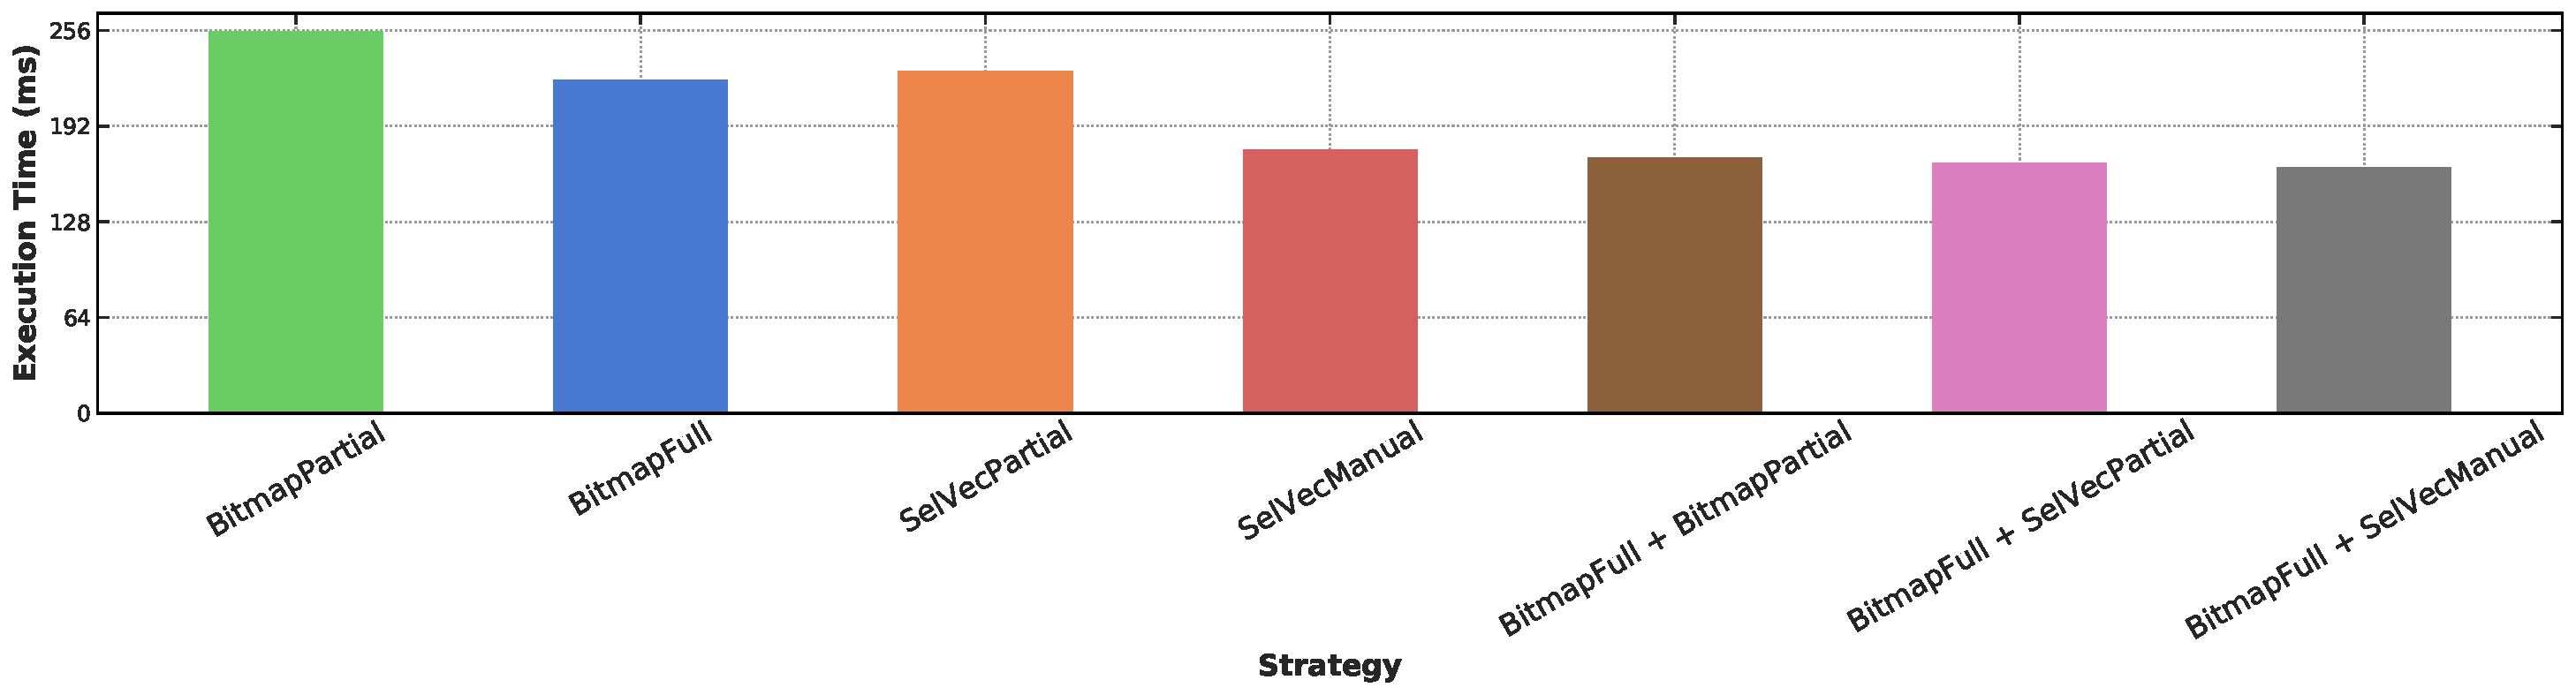
\includegraphics[width=0.9\linewidth]{eval/q6_bench.pdf}
 \caption{Total running time.}
  \label{fig:q6_bench}
\end{subfigure}%

\caption{\textbf{Q6 Performance}. The \texttt{+} notation indicates mixed strategies.}
\label{fig:q6_perf}
\end{figure}

\cref{fig:tpch_q6} shows the SQL code of the Q6 query. Its \texttt{WHERE} contains five SLDP filters, and its \texttt{SELECT} one arithmetic SLDP projection followed by an aggregation. For all vectors, the second filter leads to a selectivity below $0.15$, triggering a threshold-based switch. Thus, our decision tree favors a mixed strategy: BitmapFull at high selectivities, and SelVecManual at low selectivities.

The results are shown in \cref{fig:q6_perf}. \cref{fig:q6_optimized} shows the running time of the primitives we optimized. This graph confirms the necessity of the caveat we raised in \cref{mixedcompute}: the cost of converting from Bitmaps to SelVecs makes BitmapFull+SelVecManual slightly more expansive than BitmapFull+BitmapPartial by $0.3\%$, even though SelVecManual performs better than BitmapPartial on the individual primitives in this query. This difference is insignificant, so our decision tree does not take it into account. The BitmapFull+SelVecPartial strategy also suffers from the conversion overhead, but the difference only amounts to $2\%$. All mixed strategies perform better than non-mixed ones. BitmapFull+BitmapPartial and BitmapFull+SelVecManual are faster than BitmapFull by $1.3\times$ because Full Compute becomes wasteful after the selectivity drops below $0.15$. The SIMD SelVecManual strategy is slower by $1.04\times$ because it is only suboptimal in the first two filters of the \texttt{WHERE} clause. The SISD Selective Compute strategies BitmapPartial and SelVec Partial are slower by $1.6\times$ and $1.4\times$ because they do not take advantage SIMD instructions for SLDP operations.

\cref{fig:q6_bench} shows the total running time that includes the side-effect-full aggregation primitive. This primitive only accounts for a small portion of the running time, so we do not observe the slowdown caused by AVX512 registers. In SLDP-dominated queries like Q6, the benefits of AVX512 outweigh its disadvantages.

\section{Q4: Low Selectivity, Inefficient Data Parallelism}
\label{q4section}
\begin{figure}[t!]
    \centering
    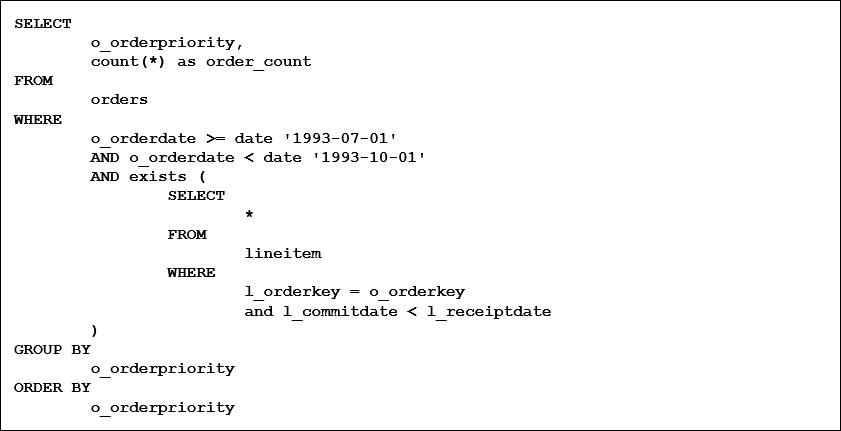
\includegraphics[scale=0.5]{images/TPCH-Q4.png}
    \caption{\textbf{The TPCH Q4 query.}}
    \label{fig:tpch_q4}
\end{figure}


\begin{figure}[t!]
\centering
\hspace*{\fill}% 
\begin{subfigure}[t]{.8\linewidth}
 \centering
 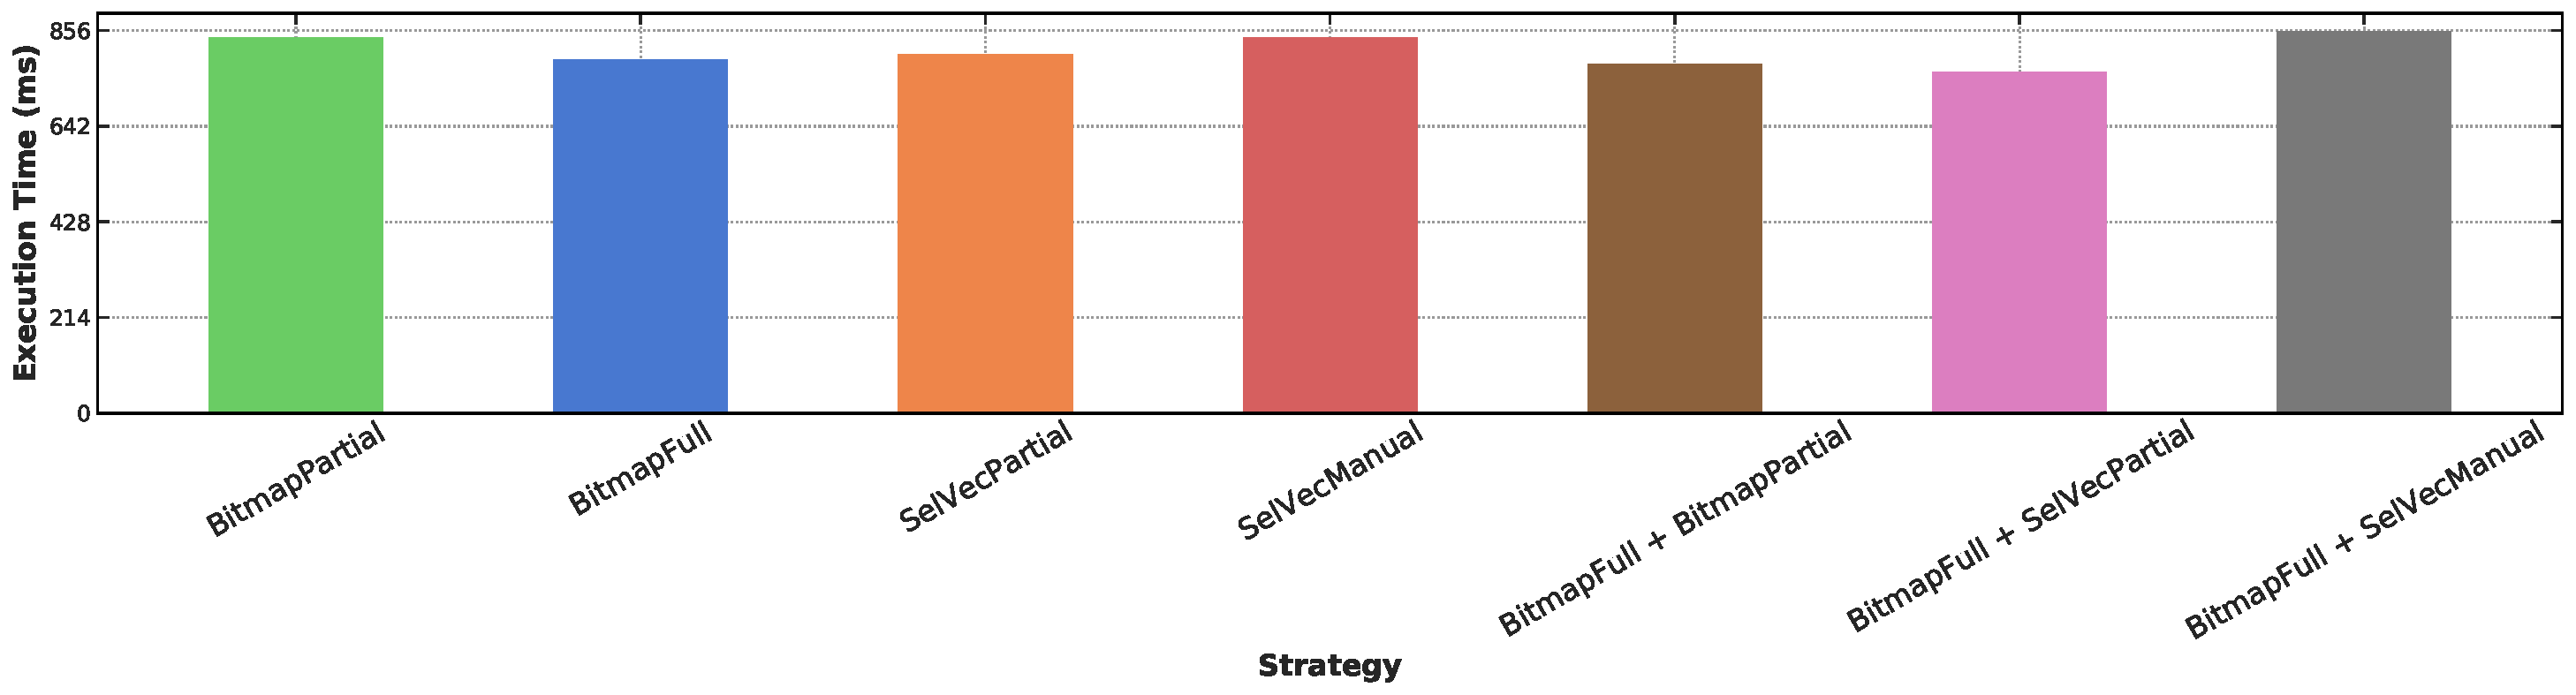
\includegraphics[width=0.9\linewidth]{eval/q4_optimized.pdf}
 \caption{Running time of side-effect free primitives.}
  \label{fig:q4_optimized}
\end{subfigure}
\hspace*{\fill}%
\vspace*{8pt}%

\hspace*{\fill}%

\begin{subfigure}[t]{.8\linewidth}
 \centering
 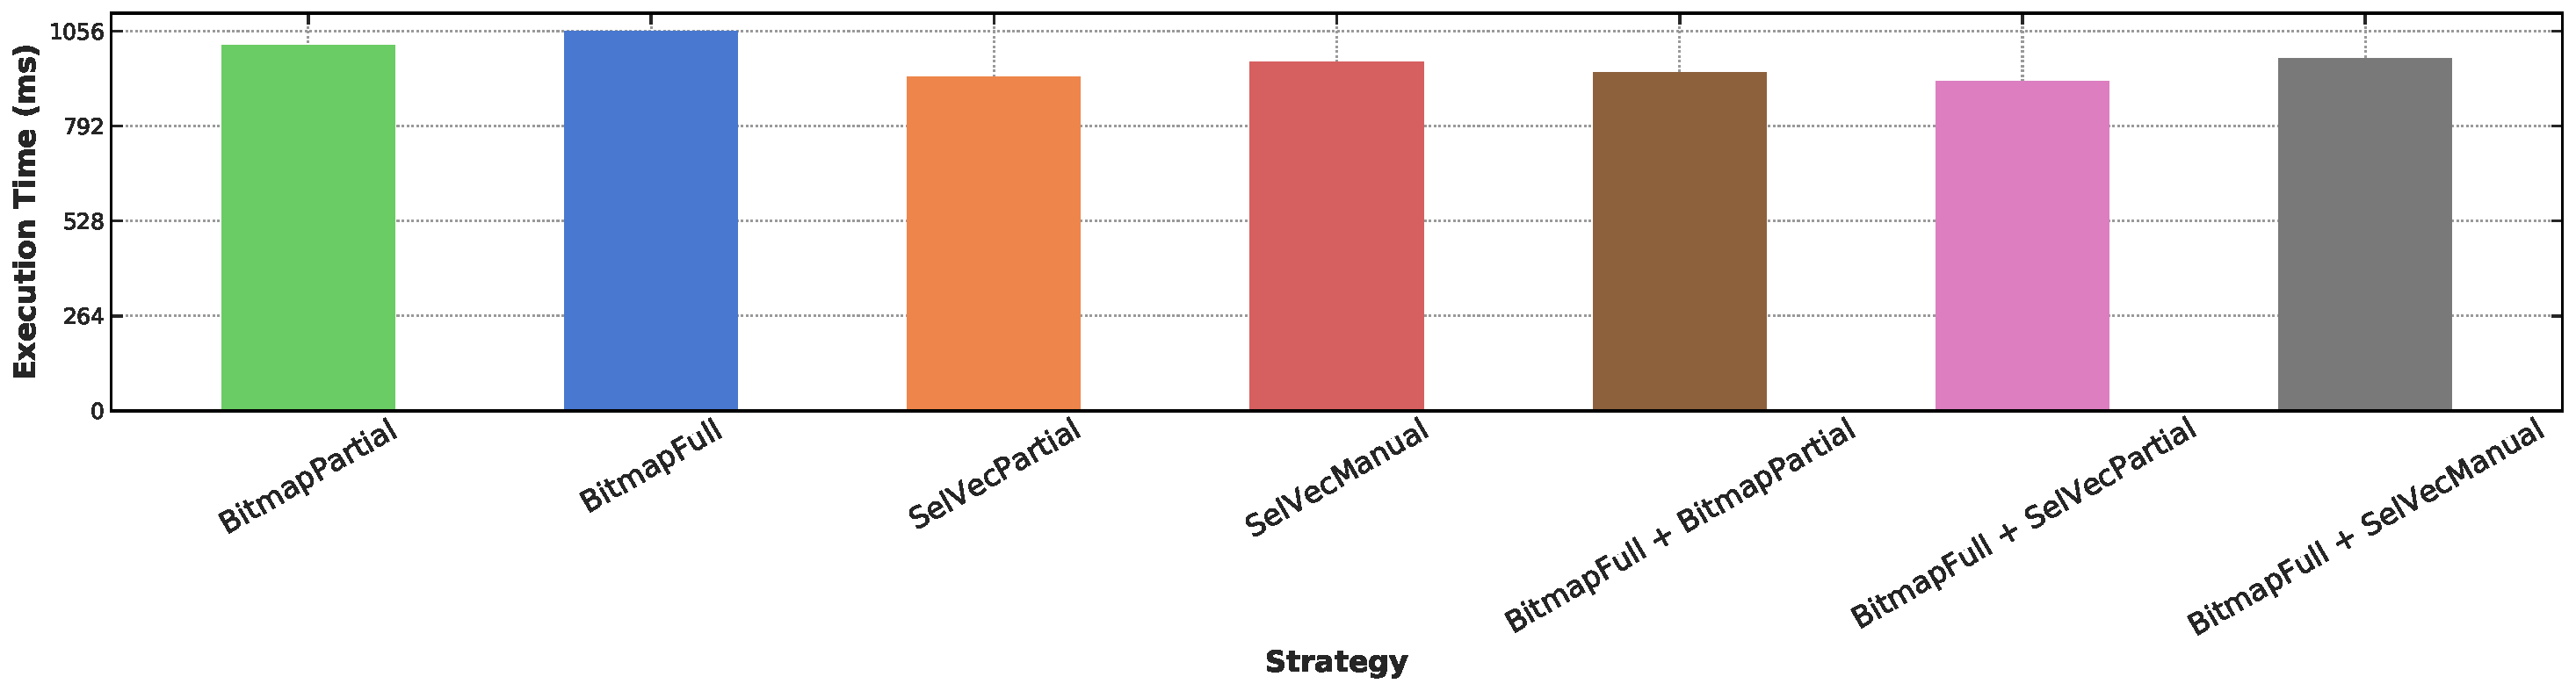
\includegraphics[width=0.9\linewidth]{eval/q4_bench.pdf}
 \caption{Total running time.}
  \label{fig:q4_bench}
\end{subfigure}%
\caption{\textbf{Q4 Performance}}
\label{fig:q4_perf}
\end{figure}

\cref{fig:tpch_q4} shows the SQL code of the Q4 query. It is a join of two tables (\texttt{lineitem} and \texttt{orders}) followed an aggregation and an order-by operator. The join's left side (from the \texttt{orders} table) has two SLDP filters that reduce the selectivity to $0.3$ and $0.1$, respectively, and an SLDP hashing primitive before insertion into the join hash table. Its right side (from the \texttt{lineitem} table) has a filter with a selectivity $>0.6$ and a join probe that contains the multiple primitives shown in \cref{fig:probe_example}. Although the probe's hashing primitive is an SLDP operation, its other primitives contain multiple indirect lookups (e.g., accessing hash table entries or the keys within those entries for exact comparison). Because these operations are called in a loop to find all potential matches during the join, they constitute the bulk of the running time. Unfortunately, their data-parallel versions are inefficient. For example, the comparison primitive, which we manually implemented for the SelVecManual strategy, contains three \texttt{gather} instructions: one to collect the keys from the right side of the join, one to collect the hash table entries, and one to collect the keys within the hash table entries for comparison. SIMD instructions can cause performance degradations in these primitives. Thus, we predict that we should use BitmapFull to perform the SLDP filters and hashing, then switch to using SelVecPartial, not the SIMD SelVecManual, for the complex primitives within the join probe.

The results are shown in \cref{fig:q4_perf}. \cref{fig:q4_optimized} shows the running time of the primitives we optimized. Our predicted strategy, BitmapFull+SelVecPartial, is indeed the optimal one, closely followed by BitmapFull+BitmapPartial, which also switches from SIMD to SISD code for complex primitives. Notice the performance degradation caused by SIMD vectorization, as mentioned in \cref{inefficientsimd}. Unlike the previous queries' results, BitmapFull+SelVecPartial performs better than the BitmapFull+SelVecManual by $1.1\times$ because the latter relies on SIMD vectorization for complex primitives. BitmapFull is also slightly worse (by $1.04\times$). Its performance degradation is attenuated by the fact that it requires fewer \texttt{gather} instructions than SelVecManual (e.g., one instead of three in the comparison primitive), relying instead on faster \texttt{vector\_load} instructions to load all elements in a vector, whether they are selected or not. The SISD Selective Compute strategies BitmapPartial and SelVecPartial are, respectively, $1.1\times$ and $1.05\times$ worse because they do not optimize SLDP primitives. 

The results in \cref{fig:q4_optimized} mostly reflect those in \cref{fig:q1_optimized}. AVX512 registers, once again, cause a slowdown in SIMD implementations, causing, for example, BitmapFull to become slower than BitmapPartial even though they share the same code for side-effect-full primitives. Here, the disadvantages of AVX512 outweigh its benefits on the full query.

\section{Summary}
Our analysis shows that our results in \cref{chapter3} provide us with the best implementation for each query. The downside is that it requires a wide variety of variants for each primitive because any strategy can be optimal under specific scenarios. We see, however, that Bitmap only strategies (e.g., BitmapFull, or BitmapFull+BitmapPartial) perform nearly as well as the optimal ones in the queries above. Developers can thus discard the SelVec representation to save engineering effort without losing too much performance.


\chapter{Related Works}
\label{chapter5}
\section{Optimizing Analytical Queries for DBMSs}
Besides the Vectorization and Materialization model introduced in \cref{chapter1}, much work has been dedicated to optimizing analytical queries on column store DBMSs. \citeauthor{materializationstrats} studied the effect of materialization strategies (i.e. late or early materialization) on query performance \cite{materializationstrats}. All experiments in this paper use late materialization and rely on filters to keep track of valid tuples. Nonetheless, \citeauthor{materializationstrats} found that the optimal materialization strategy depends on selectivity and on the exact operations performed on tuples \cite{materializationstrats}. \citeauthor{cstore} studied compression as way to optimize both data storage and query execution in column stores \cite{cstore}. \citeauthor{abadicompression} performed an extensive evaluation of various compressions schemes \cite{abadicompression}. The experiments in \cref{chapter4} rely only on dictionary compression.

Researchers have also used SIMD vectorization to optimize relational algorithms. \citeauthor{simd1} optimized scans and nested loop joins using techniques most similar to our BitmapFullManual implementation. \citeauthor{simd2} further applied SIMD vectorization hash tables probes \cite{simd2}. \citeauthor{simdsort1} and \citeauthor{simdsort2} proposed sorting algorithms using SIMD instructions \cite{simdsort1,simdsort2}. The relational order-by operators, sort-merge joins, and sorting aggregations can all use these efficient sorting algorithms.

\citeauthor{ibm_blu} and \citeauthor{simdscan} combined this body of work and built full commercial DBMSs using column stores with compression and SIMD vectorization techniques to optimize table scans \cite{ibm_blu,simdscan}. \citeauthor{orestis_bitmap} further built a system using SIMD vectorization on all relational operators \cite{orestis_bitmap}. These systems make a static filter representation decision: Bitmaps for table scans, and SelVecs for other operations.

Along with the Vectorization Model, the current state-of-the-art execution technique is the Data-Centric Query Compilation technique pioneered by \citeauthor{hyper_llvm} \cite{hyper_llvm}.  This technique splits a given query plan into several pipelines and compiles them individually. A pipeline is a sequence of relational operators that do not materialize their result set followed by a pipeline-breaker -- an operator that does materialize its result set (e.g., to build a hash table or sort tuples). This approach's benefits are: (1) eliminate interpretation overhead by compiling specialized code and (2) maximize cache locality by keeping tuples in the registers or the L1 cache for entire pipelines. Our system uses the relaxed operator fusion technique \cite{rof}, which combines data-centric code generation with the Vectorization Model. It generates code that operates on vectors of tuples, thereby eliminating the interpretation overhead and optimizing cache locality while maintaining all the Vectorization Model's benefits.


\section{Primitive Optimization}
There has been previous work dedicated to optimizing primitives in the Vectorization Model. They mostly differ from this thesis in that they do not consider the impact of filter representation in their performance. We now discuss this work and how they relate to our proposed method.
 
\citeauthor{sompolski_vec} compared the cost of vectorization to data-centric query compilation \cite{sompolski_vec} and combined the two approaches to generate new vectorized primitive at runtime, which is the method we use in \cref{sldpsection}. Using only the SelVec representation, the authors compare vectorized primitives' performance under various compute strategies (e.g., Full versus Selective Compute, Conditional versus Unconditional Store). They, however, do not provide a way to switch between these strategies. 

\citeauthor{everything_vectorized} performs a similar analysis for whole queries in addition to individual primitives \cite{everything_vectorized}. They developed a SIMD implementation of primitives using Selection Vectors, just like our SelVecManual strategy. Like ours, their implementation was effective on compute-heavy queries (e.g., Q6 in \cref{q6section}) and ineffective on memory access-heavy queries (e.g., Q4 in \cref{q4section}).

\citeauthor{miro_adapt} recognized the importance of switching compute strategy at run-time \cite{miro_adapt}. For each operation, the authors implement several \textit{flavors} (i.e., different ways to perform the same operations). They then use reinforcement learning (RL) to switch between the best \textit{flavors} dynamically at runtime. This approach is more general than our micro-benchmarks because it takes into account changes in system load. SelVec is the only representation considered, limiting the range of adaptivity on Update tasks. Besides, our decision tree provides more explainability than RL techniques. As future work, we could employ a similarly dynamic strategy to determine our thresholds.

\chapter{Conclusion}
\label{chapter6}
This work analyzed the impact of filter representation (i.e., Bitmap vs. SelVec) and compute strategy (i.e., Full vs. Selective Compute) on the performance of the vectorized primitives in an in-memory analytical DBMS. We identified the factors that influence performance: number of tuples processed, iteration logic, and core operation time per tuple. We explained how each combination of representation and compute strategy balances between these three factors. Full Compute has the cheapest iteration logic, processes all tuples, but spends less time on each tuple when SIMD vectorization is possible. Full Compute is, however, only available with Bitmaps on Update primitives. Selective Compute with SelVecs has a cheaper iteration logic than Selective Compute with Bitmaps, and is more amenable to SIMD vectorization. We confirmed these observations with several micro-benchmarks, and created a decision tree to help systems developers find the optimal implementation of arbitrary side-effect-free primitives. Finally, we showcased the benefits of our analysis on OLAP queries with multiple primitives and consistently achieved the best performance. Our performance gains over the best techniques that do not adapt filter representation and compute strategy can be up to $1.3\times$.

%\appendix
%\include{appendix}

\backmatter

%\renewcommand{\baselinestretch}{1.0}\normalsize

% By default \bibsection is \chapter*, but we really want this to show
% up in the table of contents and pdf bookmarks.
\renewcommand{\bibsection}{\chapter{\bibname}}
%\renewcommand{\bibpreamble}{This text goes between the ``Bibliography''
%  header and the actual list of references}
\bibliographystyle{plainnat}
\bibliography{citations} %your bib file

\end{document}
